%!TEX root = ../physical-olympics-2.tex
\chapter{静力学}

以运动学和动力学理论为基础,\,时不时地,\,我们发现一些典型的现象,\,包括:
\begin{itemize}
	\item 不管体系多么复杂,\,能量函数对其行为似乎起决定性的作用.
	\item 似乎总是能够从不同的体系中抽象出它的一个特征数字:\,自由度.
	\item 约束越多体系约复杂,\,它的未知约束力越来越多,\,但是多到一定程度体系只剩下一个自由度了反而用能量守恒就能够解答大多数问题.
\end{itemize}

这些现象无疑是紧密联系的,\,值得研究的.\,事实上我们要做的就是以之前的所有动力学定律为依据进一步展开讨论.\,再从头开始建立新的理论:\,先讨论运动的描述,\,再单独研究力的特性.\,最后合到一起,\,看看这能让我们得到什么.

新理论,\, 新思想,\, 新图像.\,在本章节的学习过程中,\, 如果感到疑惑,\, 大抵都是复杂的数学推导掩盖了背后的物理目的.\, 希望读者先记住两点:\,一是,\,我们要做的是把以前对质点,\,刚体和对质点系列的选取自然坐标(大抵是直角座标)而列的部分定理修改为改用广义坐标来描述,\,过程中的所有步骤都是为这个目的来服务的.\, 二是,\,本着``能量函数的形式''就决定``体系的一切结构与演化''的观点,\,我们就能找到一个明确的方向.\,无论是从结果上还是从细节上,\,我们将会多次参考这种想法.

\section{约束}
所谓\emph{约束}(constraint)就是对运动的限制.\,有时,\,物体发生直接的接触,\,或是一个物体在另一个物体表面滑动或是滚动,\,这种情况约束实际上就发生了;\,有时,\,约束通过往往是轻质\footnote{后面就能理解,\,这样才不会占用新的广义坐标,\,因为它不带来任何能量}的绳,\,直杆或曲杆,\,套筒,\,无摩擦的铰链等等去连接两个乃至多个物体,\,这样那些物体之间实际上也存在约束,\,偶尔我们也会把连接它们的机构直接叫做约束.

之所以把它们叫做约束,\,是因为它们产生了两个共同的结果,\,一是\emph{约束方程}(equation of constraint),\,二是\emph{约束力}(force of constraint).\,根据前者的运动学效果\footnote{根据后者的动力学效果还可以分为理想和非理想约束,\,见后面小节平衡问题:\,虚功原理},\,我们把与约束分为以下类别:

\subsection{约束分类}

无论是挂在天花板下的小球,\,还是``鹰击长空,\,鱼翔浅底'',\,都给我们以\emph{单边约束}(unilateral constraint)的图像.
\begin{figure}[H]
\centering
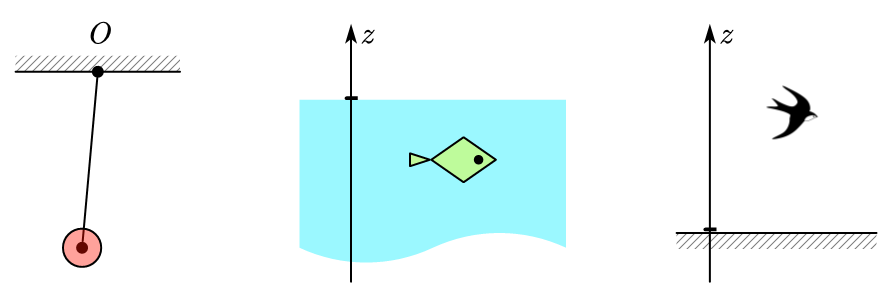
\includegraphics[width=14cm]{image/6-2-1.png}
\caption{可解约束}
\end{figure}

其中,\,	小球的位置符合$x^2+y^2+z^2\leq l^2$,\,鱼的位置符合$z\leq 0$,\,鸟则是$z\geq 0$.

更简单的例子还包括两个物体表面发生接触(滑动或滚动)的情况.\,此时两物可能会脱离接触,\,比如在半球面顶点上滑下来的质点.\,这些所有约束的典型特点,\,从约束方程上看都是一个单边不等式:
\[F\geq 0\quad {\rm or}\quad F\leq 0\]

如果不等式取等号,\,那么可以认为对物体运动的限制客观存在,\,从而会相伴相生约束力.\,但是如果运动到不等号成立了,\,比如上面三种情形中,\,绳子松弛了,\,鱼没有在表面游鸟也没有在地面走,\,那么其实原则上也不存在任何对运动的限制.\,称作约束被``解除''了.\,所以单边约束也可以称作可解约束.\,显然为了简单起见,\,我们可以把这一类问题分解为严格符合约束和没有约束两种情形来等效.\,这实际上构成了不可解的\emph{双边约束}(bilateral constraint)模型.

所谓双边约束就是把之前的单边的约束的不等式进行等式化,\,比如$x^2+y^2+z^2= l^2$就对应着把可弯曲的轻绳替换为了不可弯曲的轻杆.\,而后两个问题就变成了$z=0$,\,即不能让物体陷入也不能让物体脱离的平面约束.

故,\,针对这一类分类模式,\,双边约束显然才是``有效''的部分.\,故本书以后所有约束都指双边的.

继续根据约束的不同特点分类,\,我们就产生了两种可行的依据与分法:

一是,\,根据约束的可积性来分为\emph{完整约束}(holonomic constraint)和\emph{非完整约束}(nonholonomic constraint).

我们发现,\,一个体系的运动由若干\emph{广义坐标}(general coordinates)和它们的导数---\emph{广义速度}(general velocity)来描述.\,比如一个转盘就可以由转角$\varphi$来描述其处在的几何位置\footnote{注意,\,$\varphi$与$\varphi+2\pi$描述的位置在几何上没有区别,\,仅仅是在运动的不同过程中发生,\,一般认为达到后一个位置就是回到了初始位置(运动经历一个周期).},\,而角速度$\dot{\varphi}$来描述转动快慢.\,从而约束,\,作为对运动的限制,\,也就是应当关于这些量的方程.

但是无可辩驳的是,\,在约束发生时这一类方程,\,至少在最初被确定下来的形式下分为两大类,\,一是不含广义速度的\emph{几何约束}(geometric constraint),\,二是含广义速度的\emph{微分约束}(differential constraint).

举三个例子:

A.\,一个圆盘状的冰球本来由盘心的$(x,\,y,\,z)$和盘面方向,\,即垂直盘面的单位法向量$(\cos\alpha,\,\cos\beta,\,\cos\gamma)$构成其广义坐标,\,后面的描述方法用到了方向余弦.\,即使盘并没有被地面约束,\,三个方向余弦也要满足:
\[\cos^2\alpha+\cos^2\beta+\cos^2\gamma=1\]

现在盘到了地面(光滑冰面)上,\,更是要满足:
\[z=0\quad,\quad \alpha=\beta=\frac{\varphi}{2}\quad,\quad \gamma=0\]

这些都是几何约束.

B.\,一个半径为$R$的轮子沿$x$方向单纯地在地面做纯滚动.\,本来在没有地面之前,\,轮子由水平竖直坐标$(x,\,z)$以及自转角$\varphi$描述.\,但是,\,在有了地面做约束以后,\,就需要满足接触条件和纯滚条件(第一章学过):
\[z=0\quad ,\quad \dot{x}=R\dot{\varphi}\]

第一个约束是几何约束,\,第二个便是微分约束.

\begin{wrapfigure}[17]{o}[-10pt]{5cm}
\centering

\includegraphics[width=5cm]{image/6-2-6.jpg}
\caption{独轮车}
\end{wrapfigure}
C.\,考虑一个踩着独轮车在地面上运动的小丑,\,并忽略运动的一些细节,\,认为小丑仅仅由其水平面上坐标$(x,\,y)$和面朝方向$\theta$描述.\,且要求轮子在地面上做纯滚动,\,轮子滚动方向就是小丑面朝方向.\,描述轮子还需已知自转角$\varphi$,\,轮子半径依然为$R$.\,这些就是描述这个体系的所有广义坐标.\,那么客观地看这里有两个限制关系:
\[\frac{\dot{y}}{\dot{x}}=\frac{\sin\theta}{\cos\theta}\quad,\quad \sqrt{\dot{x}^2+\dot{y}^2}=R\dot{\varphi}\]

两个都是实打实的微分约束.

之所以称作微分约束,\,往往是因为这些约束一般都可以对广义速度齐次化,\,尤其是可以一次齐次化,\,B中的例子已经是关于广义速度$\dot{x},\,\dot{\varphi}$的一次线性组合等式了,\,C的例子也可以化为:
\[\dot{x}=R\cos\theta\dot{\varphi}\quad,\quad \dot{y}=R\sin\theta\dot{\varphi}\]

这样我们就可以在等号左右同时乘以$\ud t$,\,写成对各个变量变化微元之间的``约束''或``限制'':
\[{\rm Case\; B}:\quad \ud x=R\ud \varphi\]
\[{\rm Case\; C}:\quad \ud x=R\cos\theta\ud \varphi\quad;\quad \ud y=R\sin\theta\ud \varphi\]

这样就避免了广义速度的引入,\,依然是广义坐标之间的制约关系,\,只不过各个量不全是坐标本身,\,还含有当下状态到下一个状态间坐标的微分.

那么约束的完整性也以上两种约束是什么关系?\,我们需要注意到,\,在B中的那个约束其实是可以积分的.\,约束方程的成立就意味着:
\[x-R\varphi=x(0)-R\varphi(0)={\rm Const.}\]

这样岂不就退化为几何约束了吗?\,的确,\,像这样的微分约束与一个几何约束``等效''.\,从而我们把几何约束和可以用微分约束等效出来的几何约束一同称作完整约束.\,如果一个体系内所有约束都是完整约束,\,那么这样的体系称作\emph{完整体系}(holonomic system).\,后面我们就会发现,\,分析力学中的很多主要结论都有体系必须是完整体系的要求.

反之,\,C就不是一个完整体系了,\,因为体系含有不可积分的微分约束.\,任何看出这一点来的?\,设想通过某种积分的方式我们得到了体系的一个几何约束:
\[F(x,\,y,\,\theta,\,\varphi)=0\]

这蕴含的结果马上就会招致一个矛盾.\,对于几何约束,\,例如在B中的后一个化为的$x-R\varphi={\rm Const.}$,\,总是有经历一个复杂的过程如果$x$复原了,\,$\varphi$也会随之复原.\,这里也一样,\,如果假定以上几何约束存在,\,$F$至少``真正''含有$(x,\,y,\,\theta,\,\varphi)$四个变量之一,\,不妨设是$\varphi$\footnote{其它可能性请读者自己琢磨.}.\,那么如果在一个过程中$x,\,y,\,\theta$均复原,\,那么前后都满足约束方程的话$\varphi$一般就只有有限个解,\,更特殊地,\,必然要求也回到初态发生复原.\,然而,\,联系一下实际的物理情景便可以明白,\,小丑完全有能力让自己的位置回到初始位置,\,面朝方向也归位,\,同时轮子转过一个任意大小的角度的:\,只需要沿着半径或大或小的圆周转圈即可.\,从这一点上我们就可以发现这样的约束是不可能积分化为几何约束的非完整约束.

进一步观察我们还能发现,\,在C问题中$(x,\,y,\,\theta,\,\varphi)$四个变量具有某种``全局独立性'',\,我们总是有办法把任意的两个$(x_1,\,y_1,\,\theta_1,\,\varphi_1),\,(x_2,\,y_2,\,\theta_2,\,\varphi_2)$作为初末态用过程进行连接.\,但是我们决不要因此而认为这几个变量之间因此就彼此独立不会相互制约,\,因为约束方程客观存在,\,也就是说,\,考虑任一个状态下一时刻发生的位移$(\ud x,\,\ud y,\,\ud \theta,\,\ud \varphi)$,\,它们在``局域''看来并不具有独立性而是有相关性.\,这种\emph{局部处处成立}(locally holds everywhere)但\emph{全局不生效}(globally invalid)的行为是出于较深刻的拓扑学和分析学的原因\footnote{位形-微分流形上约束对应的矢量场间具有不为零的李导数.}.\,需要加以留心.

第二种分类方式则更加清晰明了.\,它取决于约束方程本身含不含时.\,例如在之前的绳端系球,\,以及在上面的C中的一约束方程中:
\[x^2+y^2+z^2=l^2 \quad;\quad \ud x=R\cos\theta\ud \varphi\]

它们都是不含时间的.\,从而称为\emph{稳定约束}(scleronomic constraints)\footnote{来自希腊语``坚硬'':  \begin{greek} skle'os\end{greek}}.\,但是它们对应着还存在类似的,\,\emph{非稳定约束}(rheonomic constraints)\footnote{来自希腊语``流动'':  \begin{greek} <r'ew\end{greek}}的版本,\,一种可能的情况如下:
\[x^2+y^2+z^2=(l+vt)^2 \quad;\quad \ud x=(R+vt)\cos\theta\ud \varphi\]

它们就表示绳子还在不断变长或者轮子半径在不断膨胀的新的问题.

与之前的完整非完整体系造成的区别不同,\,也许在牛顿的力学体系中处理一个非完整约束体系和非稳定约束体系的难度是相当的:\,都要进行细致的受力分析,\,能量守恒不成立或者虽然成立但用处不大.\,但是在分析力学中,\,一个体系即使约束非稳定也是与稳定约束一样适用于大多数结论的.\,分析力学的方法在求解非稳定但完整的理想约束体系中是一大利器.

\subsection{广义坐标与自由度}

拥有了约束的观点,\,便很好理解广义坐标之间的独立性的概念.\,\emph{自由度}(DOF,\,degree of freedom)也正是基于这一点而产生.\,它的定义是:\,考虑所有约束条件都成立的前提下,\,体系可以独立改变的坐标微分个数.

一般来说,\,在三维空间中(以下所有结论在二维或高维空间中都得重新讨论),\,在把一个体系的所有存在的约束都完全解除之后,\,体系可能由质点,\,线状刚体或者非线状刚体组成.\,那么直接地我们给出或者规定:\,质点的自由度为3,\,非线状刚体的自由度为6,\,线状刚体的自由度为5.\,这一点待会就可以验证.\,而一个体系若包含$a$个质点,\,$b$个线状刚体,\,$c$个非线状刚体.\,而如果约束的引入为体系带来了$r$个独立的约束方程(几何约束或微分约束),\,显然根据自由度的定义,\,体系独立变化的广义坐标的数目降为:
\[s=3a+5b+6c\quad \longrightarrow \quad f=s-r\]

这个$f$就是最终的自由度的个数.

质点的自由度为3自然是最好理解的.\,无论是用直角坐标,\,球坐标还是柱坐标,\,互相独立的坐标个数都是3.\,而它们之间又不存在任何制约关系.

如果我们把两个质点用一个刚性棍连接,\,就会带来一个距离不变的约束.\,体系自由度变为:
\[f=2\cdot 3-1=5\]

这实际上就是线状刚体的自由度数.\,因为只要确定好线状刚体上的两个点的$6$个坐标,\,那么实际上就构成了对刚体的完整描述:\,每一个质元的位置都可以简单找到.\,而这六个坐标又有一个约束关系,\,从而自由度为5.

但是非线状刚体就更复杂.\,既然非线状必然能够在刚体上找到三个不共面的固连点.\,只要确定好这三个点的9个坐标就能确定整个刚体的位形.\,但是这三个点之间两两距离不变,\,存在三个独立的约束方程,\,所以自由度数变为:
\[f=9-3=6\]

\begin{wrapfigure}[13]{o}[-10pt]{7cm}
\centering
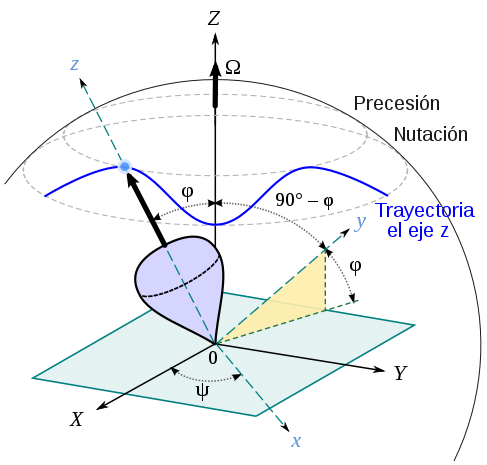
\includegraphics[width=7cm]{image/6-2-2.png}
\caption{刚体的三自由度转动}
\end{wrapfigure}
为什么线状刚体不能作为非线状刚体的特例而也具有相同的6自由度呢?\,比如一个陀螺,\,作为一个刚体分析一般为认为它有三个平动自由度和三个转动自由度.\,如果陀螺做定点转动,\,它的三个转动自由度就被简单地隔离了出来:\,它们是自转,\,进动和章动.\,但是我们不能指望一根线状刚体来自转:\,自转进行一个角度,\,对应的状态却实际上与之前的状态没有本质区别.\,更重要地是反映在能量上,\,自转既没有带来动能,\,也没有带来势能的改变,\,从而自转角根本就是一个冗余的\emph{内禀自由度}(intrinsic DOF),\,不会参与问题的讨论过程中.

从而以上论断也将基于一个基本事实:\,质点和线状刚体是真正理想的,\,现实模型:\,小球,\,细棍更精细的模型当然是6自由度的刚体,\,甚至更高自由度的质点系,\,连续体模型.

清楚了体系的基本组成部分的原始自由度数.\,我们再把视野转向常见的约束上来.

要注意,\,约束的个数这样一种说法的歧义性.\,有时候我们发现体系有$r$个独立的约束方程,\,从而说体系存在$r$个约束.\,但是有时候我们指的是有几个机构在制约着物体的运动.\,两者是有区别的,\,我们保留前者的称呼,\,后者的个数叫做约束物的个数.

Case1.\,如果用一个面来限制质点的运动,\,那么约束的个数是1.\,如果质点是一颗珠子被穿在一条空间曲线上,\,那么尽管约束物只有一个,\,但存在两个约束.\,这是因为平面和曲线方程分别是:
\[{\rm Surface:} \quad F(x,\,y,\,z)=0 \quad;\quad {\rm Curve:} \quad \left\{ \begin{matrix} F(x,\,y,\,z)=0\\ G(x,\,y,\,z)=0\end{matrix}\right.\]

这也正构成了两种情况下的约束方程.
\begin{figure}[H]
\centering
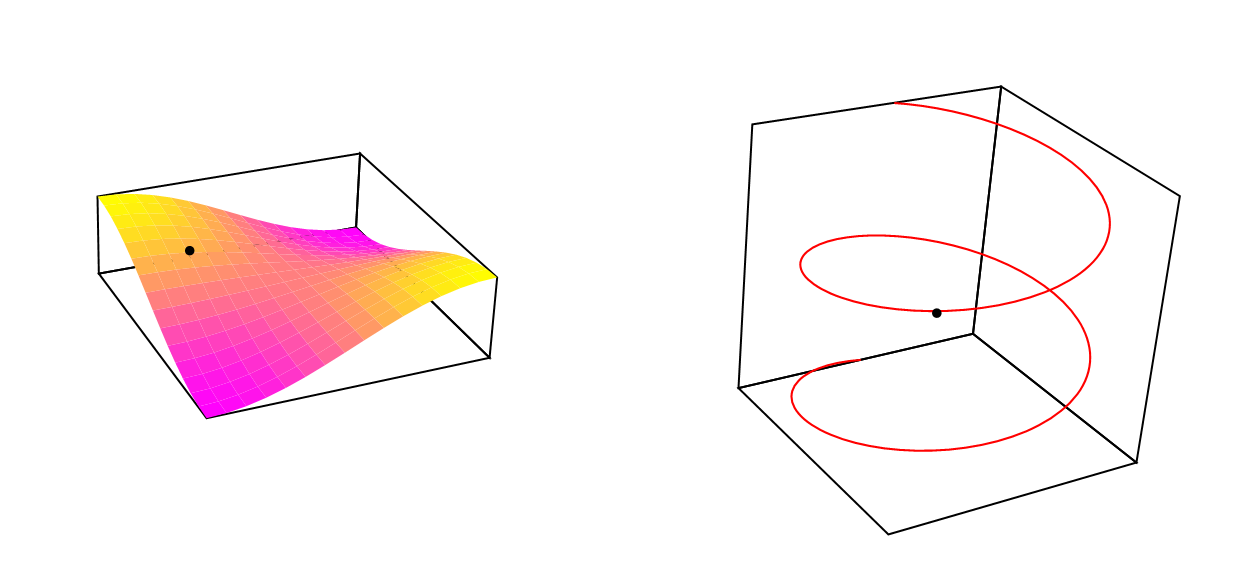
\includegraphics[width=14cm]{image/6-2-3.png}
\caption{面约束和线约束}
\end{figure}

Case2.\,但是,\,如果面和线是绝对粗糙的,\,那么质点就动弹不得.\,这样带来的约束个数,\,显然两种情况都有三个.

Case3.\,用绳子和杆子的两端连接两个物体,\,对应的约束个数显然是1.\,就是说那两个点之间的距离为一个常数.

Case4.\,如果绳子还绕过了滑轮,\,那么原则上每一段绳带来一个约束减少一个自由度.\,例如坐标为$(x_1,\,y_1,\,z_1)$的质点连接的绳(长$l$)绕过坐标为$(x_2,\,y_2,\,z_2)$的滑轮(视作质点)与坐标为$(x_3,\,y_3,\,z_3)$的质点连接,\,约束方程就是:
\[\sqrt{(x_2-x_1)^2+(y_2-y_1)^2+(z_2-z_1)^2}+\sqrt{(x_2-x_3)^2+(y_2-y_3)^2+(z_2-z_3)^2}=l\]

Case5.\,而不同于用两段绳分别连接12和23,\,这样就会带来两个约束.\,区别在于前者的一段绳两个部分可以交换绳长,\,但是后者的两段绳则不能交换绳长.

Case6.\,最后还有铰链模型.\,如果仅仅是两个物体用铰链连接,\,那么结论是显然的:\,如果是平面问题,\,那么约束个数为2.\,如果是空间问题,\,那么约束个数为3.\,约束方程就是被连接的两个点具有完全一致的所有坐标.

Case7.\,但如果是$n$个物体同时连接与一个铰链上,\,那么我们只需要把第1个物体和第2个物体连接,\,再把第2个物体和第3个物体连接...\, 最终把第$n-1$个物体同第$n$个物体连接即可,\,一共进行了$n-1$次独立的连接,\,故约束个数为$2(n-1)$(平面问题)或$3(n-1)$(空间问题).
\vspace{1cm}

引入自由度的概念,\,一个重要的原因是为了更好地描述体系的运动.\,现在我们先看更复杂的情况:\,如果体系是非完整体系,\,那么事情比较难办:\,不妨设$r$个独立约束中应当有$h$个完整约束和$k$个不完整的约束.\,那么应当给予保留$f'=s-h$个广义坐标.\,体系的运动过程中,\,这$f'$个广义坐标并不能完全相互决定,\,记作$q_1,\,q_2\cdots q_{f'}$.\,但是体系任意状态的描述都只需要确定这$f'$个广义坐标的值和导数.\,比如,\,任何一个质点的$x$坐标,\,还有速度的$x$分量就必然可以用之前的量来表示.\,而还应当存在$k$个微分约束:
\[x=x(q_i,\,t)\quad,\,\quad \dot{x}=\frac{\partial x}{\partial t}+\sum_i \frac{\partial x}{\partial q_i}\dot{q_i}\]
\[f_j(q_i,\,\ud q_i,\,\ud t)=0\]
\[i=1,\,2\cdots f' \quad,\quad j=1,\,2\cdots k\]

但是如果是完整体系,\,问题就简单了,\,自由度的个数$f$就会是体系独立的坐标的个数.\,从而如果广义坐标是$q_1,\,q_2\cdots q_f$,\,它们之间就不存在约束关系了,\,体系的一切量,\,原来如果由类似于$x,\,\dot{x}$这样的量来表示,\,现在就直接是:
\[x=x(q_i,\,t)\quad,\,\quad \dot{x}=\frac{\partial x}{\partial t}+\sum_i \frac{\partial x}{\partial q_i}\dot{q_i}\quad (i=1,\,2\cdots f)\]

尤其是稳定的完整约束体系.\,那么由于约束方程不含$t$,\,那么上式就更是简化为:
\[x=x(q_i)\quad,\,\quad \dot{x}=\sum_i \frac{\partial x}{\partial q_i}\dot{q_i}\quad (i=1,\,2\cdots f)\]



\subsection{约束力与广义力}

为了简单起见,\,我们把刚体也当作多个通过约束固连在一起的质点构成的系统.\,这样体系便只含有以下要素:\,质点,\,外力,\,约束,\,质点间的内力,\,约束力(也是内力).

正过来看,\,任何一个约束都可以限制到若干质点.\,从而同时对这几个物体的运动提出单个的制约关系(自由度减1).

但是另一方面,\,每一个质点又同时可能受到若干个约束物的共同限制,\,每一个约束物就会对该质点施加一个或多个约束方程来把这个质点的运动和其他质点运动联系起来.

在牛顿力学情况下,\,我们总是喜欢分析那个质点受到的约束物给它的力的具体特征.\,这种力就叫做约束力.

约束力的最核心特征,\,就在于它是\emph{被动力}(passive force).\,直接看是找不到这么一个力的大小与方向的.\,约束力的具体值,\,是两个因素共同作用的结果:\,一方面就是约束本身的性质:\,是光滑的还是粗糙的?\,是要耗散还是甚至可以输出能量?\,但是更重要的是,\,约束力必然受到具体运动情况和体系动力学结构的影响.\,这一点很好理解:\,因为如果把某个约束解除,\,那么体系之后的运动就不一定遵从约束方程.\,那么解除约束之前的体系就正是因为约束给出来的力影响了其运动而导致其运动``回归正轨''.

基于这一点,\,就不难判断,\,质点受到``必要''约束力的个数,\,就是质点坐标参与约束方程的个数.

比如,\,被穿在光滑曲线上的质点受到的约束力必然是两个,\,再比如,\,平面问题中,\,两个用光滑铰链连接的物体会在两个方向上产生约束力,\,而如果是$n$个物体铰接在一起,\,那么期间我们如果设出$2(n-1)$个约束力就意味着个数设对了.


显然,\,如果是粗糙的曲线上有一个滑动的质点,\,曲线给质点的力应当有两个支持力和一个滑动摩擦力,\,也就是说应当是三个,\,而不是约束给出的两个.\,再比如,\,将一条长$l$的轻绳子绕过三个光滑滑轮组成一个闭合的圈.\,那么明显每个物体与之相关的约束方程只有一个.\,但是约束力似乎也得有两个拉力.

\begin{wrapfigure}[13]{o}[-10pt]{5cm}
\centering
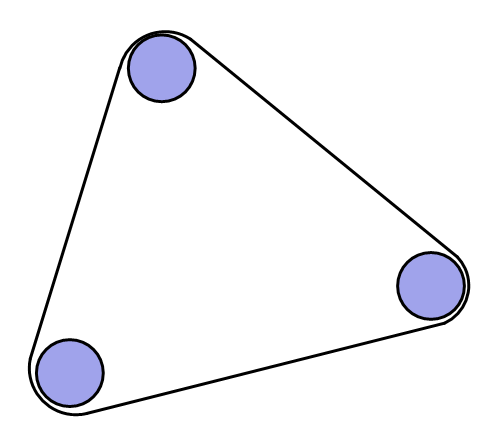
\includegraphics[width=5cm]{image/6-2-4.png}
\caption{三物体一约束}
\end{wrapfigure}
这两种情况也得分开讨论.\,第二种情况下,\,两个拉力总是相等,\,从而三个质点的受力都指向三个角平分线的交点:\,内心.\,这个约束给三个质点的力其实应当认为是两个力的合力.\,它只有沿内心与质点连线方向的分量,\,没有垂直方向的,\,可以算作一个约束力而不是两个.\,但是前者的确应当算作三个约束力.\,这是因为滑动摩擦力分量明显不是``必要的''.\,它独立于之前的两个支持力.\,也不同于之前两个支持力.

其中具体的道理还得见后面虚功原理一节的关于理想约束的推导.\,我们指出,\,在上一章讨论约束力功的时候我们提出的约束力公式,\,在这里可以直接推广.\,实际上就能得到我们一直在说的``必要''约束力.\,在一般情况下,\,如果某约束对一质点的$x$坐标产生了限制:
\[f(x,\cdots)=0\]

那么与之相伴而生的作用在质点上的约束力就必然有一项$x$分量:
\[F_x=\lambda_f\frac{\partial f}{\partial x}\]

如果还含$y$那$y$方向自然也会产生一个约束力,\,公式是一样的.\,如果含有其他质点坐标时就换那个质点的坐标来求片导数.\,注意由同一个约束方程产生的所有的约束力都共用同一个$\lambda_f$.

对于理想约束这就是全部的约束力和它要符合的形式,\,非理想约束则可能产生各种各样的其它形式的约束力.

还有一个重要概念需要先一步加以介绍.\,如果我们考虑任何一个作用在实际体系的某质点上的力$\bs{F}$,\,该质点坐标为$\bs{r}=(x,\,y,\,z)$.\,我们引入一个新的概念.\,这个力产生的在每一个广义坐标$q_i$上的广义力$Q_i$:\,其定义也相当简单,\,就是要使得下面连等式成立:
\[\ud W=\bs{F}\cdot \ud \bs{r}=\sum_i Q_i\ud q_i\]

这是希望用广义力对广义位移来做功来代替以往的矢量力对质点做功的一成不变的做法.\,我们默认体系都是稳定约束,\,那么其实该质点的任意位移,\,简单地可以用广义坐标上的位移来表示:
\[\bs{r}=\bs{r}(q_i)\quad \Rightarrow \quad \ud \bs{r}=\frac{\partial \bs{r}}{\partial q_i}\ud q_i\]

代入之前的要求就发现,\,广义力的算法为:
\[Q_i=\bs{F}\cdot\frac{\partial \bs{r}}{\partial q_i}\]
\vspace{0.5cm}

\begin{wrapfigure}[13]{o}[-10pt]{4cm}
\centering
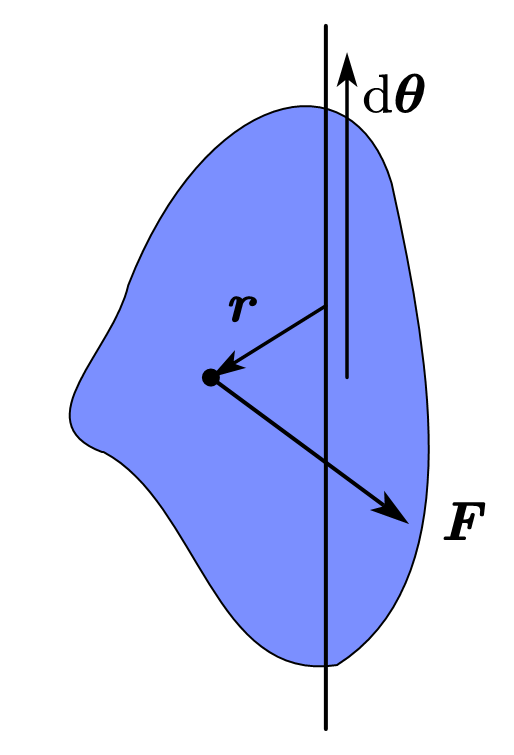
\includegraphics[width=4cm]{image/6-2-5.png}
\caption{力矩作为广义力}
\end{wrapfigure}
看两则应用:

一是刚体可做定轴转动,\,那么当刚体产生$\ud \bs{\theta}=\ud \theta \bs{e}$的转动时,\,作用在$\bs{r}$的力$\bs{F}$的作用点的实际位移为:
\[\ud \bs{r}=\ud \bs{\theta}\times \bs{r}\]

那么力的实际做功为:
\begin{align*}
\ud W  &=\bs{F}\cdot \ud \bs{r}\\
		    &=\bs{F}\cdot(\ud \bs{\theta}\times \bs{r})\\
			&=(\bs{r}\times\bs{F})\cdot\ud \bs{\theta}\\
			&=\bs{M}\cdot \bs{e}\ud \theta\\
			&=Q_\theta \ud \theta
\end{align*}

这也就是说,\,沿轴方向的力矩$\bs{M}\cdot \bs{e}$就是与角位移$\ud \theta$伴随的广义力$Q_\theta$.

\begin{wrapfigure}[17]{o}[-10pt]{3cm}
\centering
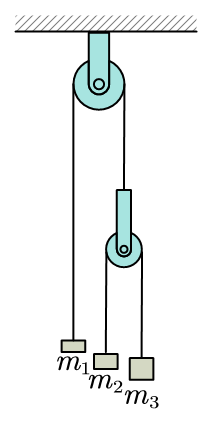
\includegraphics[width=3cm]{image/6-2-7.png}
\caption{滑轮组}
\end{wrapfigure}
再来看看在牛顿力学体系中比较基础的滑轮组问题.\,如果两个自由度分别取为:\,一.\,2,\,3挂着的动滑轮的下降与1上升的高度x;\,二.\,相对动滑轮,\,2的上升与3的下降高度y.\,那么1,\,2,\,3的向下位移就分别为:
\[s_1=-x\quad,\quad s_2=x-y\quad,\quad s_3=x+y\]

这样,\,三个重力在这两个自由度上累积的广义力就是:
\[Q_x=-m_1g+(m_2+m_3)g\]
\[Q_y=(m_3-m_2)g\]

这有什么用?\,实际上我们计算动能还可以得到``广义质量'':
\begin{align*}
T 	&=\frac{1}{2}(m_1\dot{s}_1^2+m_2\dot{s}_2^2+m_3\dot{s}_3^2)\\
	&=\frac{1}{2}(m_1+m_2+m_3)\dot{x}^2+\frac{1}{2}(m_2+m_3)\dot{y}^2+(m_3-m_2)\dot{x}\dot{y}
\end{align*}

由于产生了交叉项,\,我们再进行一次换元:
\[z=y+\frac{m_3-m_2}{m_3+m_2}x\]
\[Q_x\ud x+Q_y\ud y=\left(Q_x-\frac{m_3-m_2}{m_3+m_2}Q_y\right)\ud x+Q_y\ud z=Q_x'\ud x+Q_z'\ud z\]

从而动能和广义力变为:
\[T=\frac{1}{2}\left(m_1+\frac{4m_2m_3}{m_2+m_3}\right)\dot{x}^2+\frac{1}{2}(m_2+m_3)\dot{z}^2\]
\[Q_x'=\left(\frac{4m_2m_3}{m_2+m_3}-m_1\right)g\quad,\quad Q_z'=(m_3-m_2)g\]

这就完全与两个质点独立地受到两个恒力的动能与广义力的``结构''一致了.\,从而两个自由度的坐标二阶导数为:
\[\ddot{x}=\frac{\frac{4m_2m_3}{m_2+m_3}-m_1}{\frac{4m_2m_3}{m_2+m_3}+m_1}g\quad,\quad \ddot{z}=\frac{m_3-m_2}{m_3+m_2}g\]

从而最开始的广义坐标$y$:
\[\ddot{y}=\ddot{z}-\frac{m_3-m_2}{m_3+m_2}\ddot{x}=\frac{2m_1\frac{m_3-m_2}{m_3+m_2}}{\frac{4m_2m_3}{m_2+m_3}+m_1}g\]

本题用广义力方法求解的关键好处在于:\,本来作为矢量都同向的重力,\,在转化为广义力时可以因为体系结构不同而带上正负号.\,以适应最后的结果.

\vspace{1cm}
其实,\,广义力乘广义位移等于做功的现象我们并不少见,\,不管是热学中的$\ud W=-p\ud V$,\,还是电路问题中的$\ud W=U\ud Q$,\,抑或是电磁介质问题中的$\ud W=E\ud P,\,\ud W=H\ud M$等等公式.\,全都归于统一的广义力乘广义位移这样的形式上.\,

\section{力系化简}

静力学中大量涉及到由质点,\,刚体和简单约束构成的问题.\,本节正是要针对这一类问题形成行之有效的强大工具.\,我们建立在之前的理论基础上,\,重新构建静力学过程中适用的新逻辑体系.

\subsection{静力学公理体系}

质点也好,\,刚体也好,\,其平衡都是较为简单讨论的.\,在某一个状态下,\,我们用\emph{力系}(force system)来描述它们的受力状态.\,比如刚体上受到的力系为$\mathfrak{F}$.\,一种简单的理解是,\,力系应当是一个场.\,在刚体的每一个点上都存在该点的受力情况.\,质点则只需要描述自己那点上的受力情况就行.\,而这个场,\,应当是一个矢量场:
\[\text{公理一}:\qquad \mathfrak{F}:\,\bs{f}(\bs{r})=f_x(x,\,y,\,z)\bs{i}+f_y(x,\,y,\,z)\bs{j}+f_z(x,\,y,\,z)\bs{k}\]

如果$f_x,\,f_y,\,f_z$是连续函数,\,那么这样的力系实际运用中叫做\emph{分布力系}(distributed force system).\,$\bs{f}$其实在量纲和概念上为外力的力密度.\,但是想到质点受力的描述,\,我们立马发现所有力都必须集中于一个点,\,仿佛与分布力系略有区别:
\[\mathfrak{F}:\,\{\cdots(\bs{r},\,\bs{F}_i)\cdots\}\]

\begin{figure}[H]
\centering
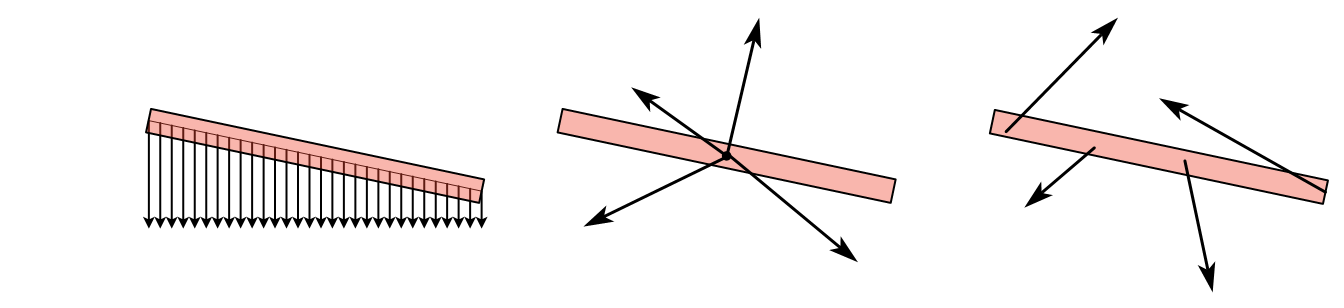
\includegraphics[width=16cm]{image/6-2-8.png}
\caption{分布力系,\,共点力系与空间力系}
\end{figure}

其中$\bs{r}$是质点的位矢.\,这样的力系可以叫做\emph{共点力系}(concurrent force system).\,事实上,\,我们也可以让刚体上若干点受到离散的作用力,\,这才是我们常说的\emph{空间力系}(spacial force system):
\[\mathfrak{F}:\,\{\cdots(\bs{r}_i,\,\bs{F}_i)\cdots\}\]

但其实两者是统一的.\,统一的关键是要引入一种广义函数:\,\emph{德尔塔函数}(delta function).\,即:
\[\mathfrak{F}_1:\,\{\cdots(\bs{r}_i,\,\bs{F}_i)\cdots\}\quad =\quad \mathfrak{F}_2:\,\sum_i \bs{F}_i\delta(\bs{r}-\bs{r}_i)\]

德尔塔函数的定义是这样的,\,如果让自变量为$\bs{\Delta}$,\,那么:
\[\delta(\bs{\Delta})=\left\{\begin{matrix}0& (\bs{\Delta\neq \bs{0}}) \\ +\infty&(\bs{\Delta= \bs{0}})\end{matrix}\right.\quad,\quad \int\limits_D \delta(\bs{\Delta})\ud \bs{\Delta}=\left\{\begin{matrix}0& (\bs{0}\in D) \\ 1&(\bs{0}\notin D)\end{matrix}\right.\]

统一为分布力系将有利于统一运算:\,如果是力个数可数的离散的空间力系,\,可以考虑两个力系的集合并:
\[\{\cdots(\bs{r}_{1i},\,\bs{F}_{1i})\cdots\}\quad \cup\quad\{\cdots(\bs{r}_{2j},\,\bs{F}_{2j})\cdots\}=\{\cdots(\bs{r}_{1i},\,\bs{F}_{1i})\cdots(\bs{r}_{2j},\,\bs{F}_{2j})\cdots\}\]

但是如果力共点了又应当去求矢量和.\,也就是说,\,本来共点力系的力就是一个三维空间中的线性代数,\,它们理所当然地定义了加法和数乘:
\[\mathfrak{Addition}:\quad \bs{F}_1+\bs{F}_2=\bs{F}\]
\[\mathfrak{Multiplication}:\quad \lambda \bs{F}_1=\bs{F}_2\]

现在就可以发现.\,第一,\,把共点力系的加法(力的叠加),\,现在就可以自然地推广到分布力系的加法来(数乘也同理).\,只需要逐点把每点处的两个力密度矢量加在一起就是合力系.\,例如,\,如果两个力系分别为$\mathfrak{F}_1:\,\bs{f}_1(\bs{r})$和$\mathfrak{F}_2:\,\bs{f}_2(\bs{r})$,\,那么:
\[\mathfrak{F}_1+\mathfrak{F}_2:\,\bs{f}_1(\bs{r})+\bs{f}_2(\bs{r})\]
\[\lambda \mathfrak{F}_1:\,\lambda \bs{f}_1(\bs{r})\]

这样就不需要分离散力系的并与共点力系的和来阐述物理上的``叠加'',\,它们本质上就是力密度分布函数的和.\,线性代数中一切应当符合的``泛性质''它也应当符合.\,其零元素就称作\emph{零力系}(null force system):
\[\mathfrak{0}:\,\bs{o}(\bs{r})=\bs{0}\]

静力学自成一套的理论核心,\,是虽然质点平衡时一定意味着合力系为零力系.\,但是在一个刚体平衡的时候,\,它依然可以对应在不同点受到不同力的一个力系.\,事实上,\,即使不平衡,\,两个不同的力系其``效果''也可以是相同的.\,以往的力学告诉我们,\,效果其实就是指产生的加速度或角加速度等运动学响应.\,但是,\,在公理化静力学的过程中,\,我们不需要关心``效果''一词的具体含义,\,而是抽象的定义一种新的关系:

这就是两个力系的\emph{等效}(equivalence),\,如果两个力系$\mathfrak{F}$和$\mathfrak{G}$等效,\,就记作$\mathfrak{F}\equiv\mathfrak{G}$.\,其实数学上有一对应的概念为\emph{等价关系}(equivalence relation),\,它需要满足以下三个条件,\,在物理观点下看是显然的:
\begin{itemize}
	\item \emph{反身性}(reflexive property):\qquad$\mathfrak{F}\equiv\mathfrak{F}$
	\item \emph{对称性}(symmetric property):\qquad$\mathfrak{F}\equiv\mathfrak{G}\quad \Leftrightarrow\quad\mathfrak{G}\equiv\mathfrak{F} $
	\item \emph{传递性}(transitive property):\qquad$\mathfrak{F}\equiv\mathfrak{G}\,,\,\mathfrak{G}\equiv\mathfrak{H}\quad \Rightarrow\quad\mathfrak{F}\equiv\mathfrak{H} $
\end{itemize}

但是还有一点十分必要,\,这样一个等价关系必须还得是\emph{同余}(congruence)的.\,即,\,它必须保持代数关系不变.\,这就构成了静力学第二公理:
\[\text{公理二}:\qquad \mathfrak{F}_1\equiv\mathfrak{F}_2\,,\,\mathfrak{G}_1\equiv\mathfrak{G}_2\quad \Rightarrow \quad \mathfrak{F}_1+\mathfrak{G}_1\equiv\mathfrak{F}_2+\mathfrak{G}_2\,,\,\lambda\mathfrak{F}_1\equiv\lambda\mathfrak{F}_2\]

这两个公理赋予力系这一个代数系统以极其规则而且性质丰富的结构.\,例如,\,我们可以定义\emph{平衡力系}(equilibrium force system)的概念:\,如果$\mathfrak{K}\equiv \mathfrak{0}$,\,即等效于零力系的力系就是平衡力系.\,那么显然任何一个力系上增减平衡力系的结果都会得到等效的力系:
\[\mathfrak{K}\equiv \mathfrak{0}\quad \Rightarrow \quad \mathfrak{F}+\mathfrak{K}\equiv \mathfrak{F}\]

那么就可以把所有平衡力系全部都找到,\,构成一个平衡力系的集合,\,称作\emph{平衡核}(kernal of equilibrium):
\[{\rm K}=\{\mathfrak{K}|\mathfrak{K}\equiv \mathfrak{0}\}\]

那么两个力系等效的充要条件就是其差在平衡核内,\,就是说如果把一个力系中的力完全做反向操作后两者就可以平衡:
\[\mathfrak{F}\equiv \mathfrak{G}\quad \Leftrightarrow \quad \mathfrak{F}- \mathfrak{G}\equiv \mathfrak{0}\quad \Leftrightarrow \quad \mathfrak{F}- \mathfrak{G}\in {\rm K}\]

最后就可以定义力系的等效类:\,所有与力系$\mathfrak{F}$等效的力系也构成了一个集合,\,记作$[\mathfrak{F}]$.\,也就是说上面的平衡核其实就是$[\mathfrak{0}]$.\,那么这个类的结构其实就是:
\[[\mathfrak{F}]=\{\mathfrak{F}+\mathfrak{K}|\mathfrak{K}\in {\rm K}\}\]

这样就把所有可能的力系的集合分解为一个一个的等效类,\,每一个集合内部的每个力系彼此之间完全等效,\,而平衡核是它们之中所有平衡力系构成的``核心''等效类.\,不同的类之间就不存在等效关系.\,每一个等效类内部的差其实都是一些平衡力系.\,两个不同的等效类中的力系差依然是一个非平衡的力系.

所以这样就把最终问题直接等效为最后一个细节:\,那就是平衡核究竟有多大?\,怎样的力系是平衡力系,\,属于平衡核?

这个问题的答案其实简单:\,那便是找到最基础的平衡力系,\,它是平衡核的\emph{生成元}(generating element).\,这就是静力学的第三公理:\,任意二力构成的,\,等大反向共线的力系全构成平衡力系,\,它是二力平衡的充分且必要条件:
\[\text{公理三}:\qquad \{(\bs{r}_1,\,\bs{F}_1),\,(\bs{r}_2,\,\bs{F}_2)\}\in{\rm K}\quad \Leftrightarrow \quad \bs{F}_1+\bs{F}_2=\bs{0}\,,\,\bs{F}_1//\bs{F}_2//(\bs{r}_2-\bs{r}_1)\]

\begin{wrapfigure}[10]{o}[-10pt]{8cm}
\centering
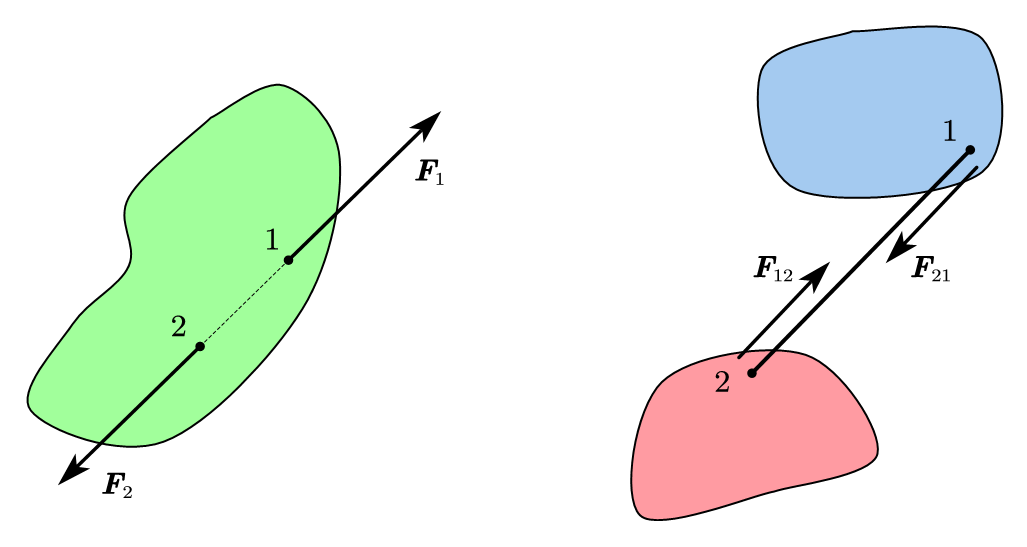
\includegraphics[width=8cm]{image/6-2-9.png}
\caption{第三公理和第四公理}
\end{wrapfigure}


这个定理又忽然把我们从分布力系的问题拉回了特殊的空间力系分析的问题,\,它们都实用且简单.\,但是从特殊到普遍,\,从二力平衡条件开始,\,一步步去探究力系是否是平衡力系的判据,\,乃至找到所有可能的平衡力系的过程可是非常细致与漫长.\,后面我们会一个推论一个推论地来完成这个过程.\,在这里我们先尚且指出另外两个通常也被认为是静力学公理的性质,\,成为我们接下来一些推理的出发点.

当我们分析一个含约束的质点,\,刚体构成的系统时,\,它们不仅受到外力,\,还要受约束力(作为内力).\,那么以前的牛顿第三定律就可以完全被静力学化也成为公理:\,如果约束发生在两个物体的两点1和2之间,\,位置分别为$\bs{r}_1$和$\bs{r}_2$.\,那么1给2的力$\bs{F}_{12}$和2给1的力$\bs{F}_{12}$就要符合:
\[\text{公理四}:\qquad \bs{F}_{12}+\bs{F}_{21}=\bs{0}\,,\,\bs{F}_{12}//\bs{F}_{21}//(\bs{r}_2-\bs{r}_1)\]

这样是否就能解决任何静力学平衡问题呢?\,对一个刚体而言这就够了.\,其力系是平衡力系自然就是平衡条件.\,然而对复杂体系的事实是:\,约束力作为被动力往往也要作为待求的量进入平衡方程.\,在约束力确定之前自然不能知道是否能平衡.\,那么如何评价含未知约束力时的平衡问题呢?\,我们规定:

\[\text{公理五}:\qquad \text{系统平衡充要条件是,\,存在一种约束力取值,\,考虑约束力后每一个部分单独平衡.}\]

它还有一个常见推论:\,由于考虑每一个部分的力系的时候是平衡力系,\,那么把这些力系进行叠加也是平衡力系,\,再考虑到成对存在的内力符合公理四,\,再由公理三,\,公理四的条件恰好让这些内力构成平衡力系.\,故扣除掉以后,\,剩下的外力力系自然也必须是平衡力系,\,也就是说如果设想整个体系等效为一个大刚体,\,那么外力就是它受到的所有力,\,此时就能得出为了平衡,\,外力就必须构成平衡力系的条件,\,因此,\,这个推论得名\emph{刚化原理}(principle of solidification).\,这是原来体系平衡的必要条件.
\[\text{刚化原理}:\qquad \text{系统平衡必要条件是外力}\mathfrak{F}\equiv \mathfrak{0}\]

\npg{1cm}

有了这些公理的基础,\,我们就可以获得十分强大的一些推论(证明过程略),\,它们都是我们进行力系化简的关键工具:
\[\text{推论一}:\qquad \text{力是滑移矢量}:\,(\bs{r}_1,\,\bs{F})\equiv(\bs{r}_2,\,\bs{F})\;\Leftrightarrow \;\bs{F}//(\bs{r}_2-\bs{r}_1)\]

从而,\,描述一个刚体上力的效果时.\,只有力的作用线是关键的.\,将一个力沿作用线滑移不改变力的作用效果.

如果把两个力系进行``叠加'',\,可以称作``合成''.\,把共点力系做矢量和也可以称作``合成''\,但是如果出现一个完整的力系恰好等效于一个单力构成的力系的情况,\,则称这个单力为力系的\emph{合力}(join force).

\begin{figure}[H]
\centering
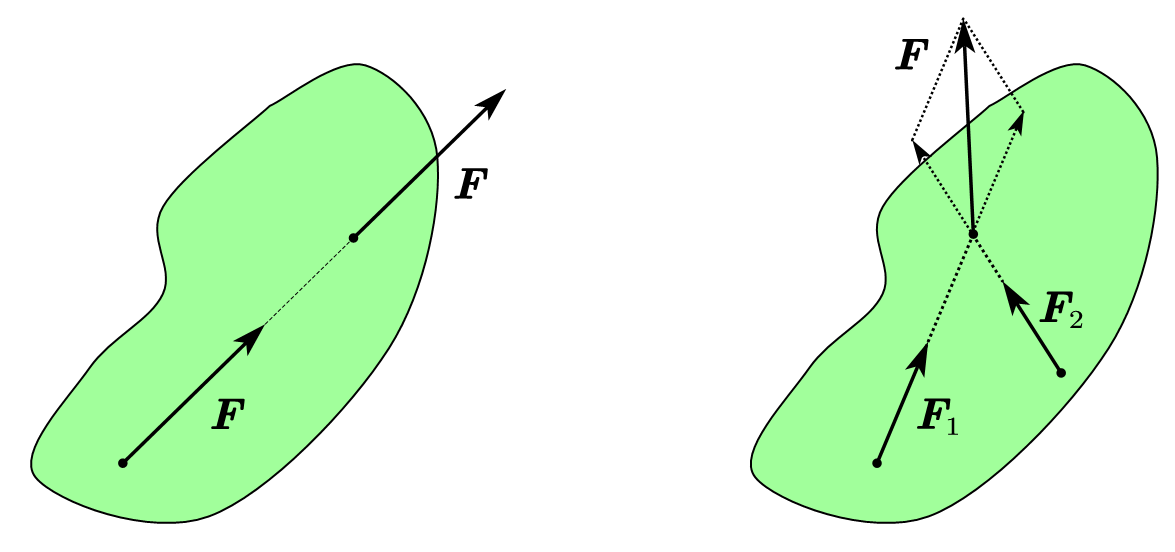
\includegraphics[width=7cm]{image/6-2-10.png}
\caption{滑移与合力}
\end{figure}

上一个推论的直接结果是:\,可以在平面力系的情形下合成任意两个非平行力,\,即非平行力求合力:
\[\text{推论二}:\qquad \text{非平行力求合力}:\,\text{如果两个力作用线交于一点,\,那么可以滑移到该点来做矢量合成求合力.}\]

\begin{wrapfigure}[12]{o}[-10pt]{6cm}
\vspace{-1cm}
\centering
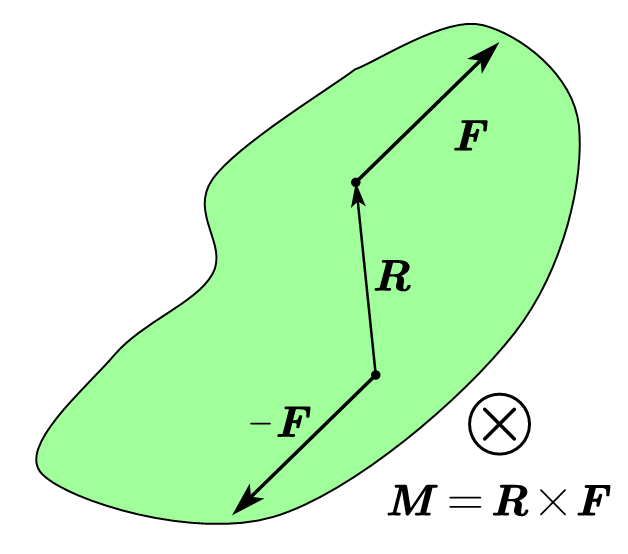
\includegraphics[width=6cm]{image/6-2-11.png}
\caption{力偶}
\end{wrapfigure}
为了求解力的非滑移的平移如何等效的问题.\,我们需要开始引入矩的概念.\,如果一个单力力系保持大小方向不变但作用在另一个点上,\,那么两个力系做差的同余类便是一个\emph{力偶}(force couple).\,最典型的情形下,\,力偶由两个力构成:
\[\mathfrak{M}=\{(\bs{r}_1,\,\bs{F}),\,(\bs{r}_2,\,-\bs{F})\}\]

力偶的特征由\emph{力偶矩}(moment of couple)来描述.\,它被定义为:
\[\bs{M}=(\bs{r}_1-\bs{r}_2)\times\bs{F}\]

可以分解为力偶的力系称作\emph{力偶系}(system of couples).\,例如如图,\,在加速运动的车厢中静止的桌子的受力就构成力偶系.\,我们把重力分解为前后脚的支持力之和,\,并分别与两个支持力构成力偶.\,摩擦力则与惯性力构成力偶.

\begin{wrapfigure}[12]{o}[-10pt]{5cm}
\vspace{-0.2cm}
\centering
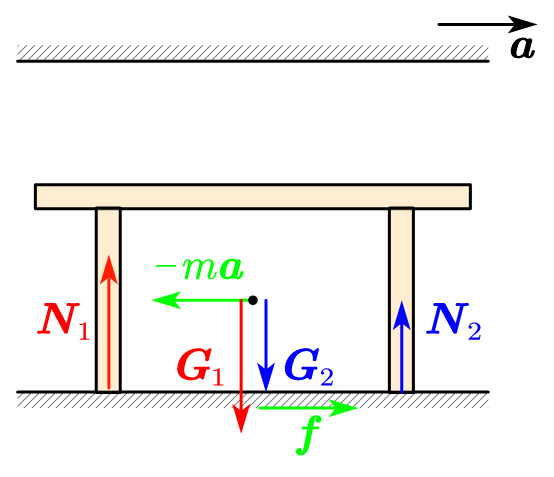
\includegraphics[width=5cm]{image/6-2-12.png}
\caption{桌子受力分析}
\end{wrapfigure}

这样一个力偶系的平衡条件是显而易见的.\,事实上,\,对力偶系的分析中,\,力偶本身是一种非定位的元素.\,只需要两个力构成的单力偶系的力偶矩一致,\,它们就是等效的.\,所以力偶系的描述方法为:
\[\mathfrak{M}=\{\bs{M}_1,\,\bs{M}_2\cdots\bs{M}_n\}\]

每一个力偶都不需要具体指定是由哪两个力组成,\,位置在哪儿.\,也正因为如此,\,力偶系描述时这些力矩都不需要支配任何作用点.\,力偶系的化简更是简单:\,直接对力偶做矢量和便是等效的.
\[\{\bs{M}_1,\,\bs{M}_2\cdots\bs{M}_n\}\equiv\{\bs{M}=\sum_i \bs{M}_i\}\]



\begin{figure}[H]
\centering
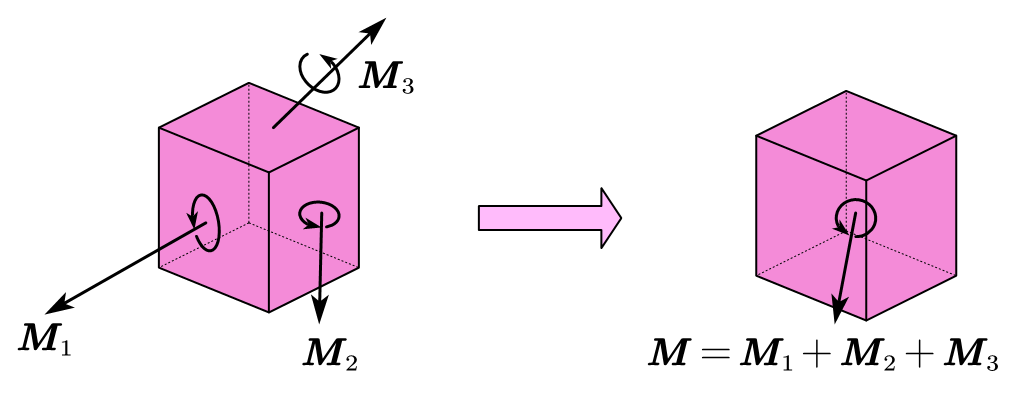
\includegraphics[width=10cm]{image/6-2-13.png}
\caption{力偶系合力}
\end{figure}
我们也把最后那个合力矩$\bs{M}$称为力偶系的合力.
现在我们可以写出共点力系和力偶系的平衡充要条件:
\[\text{推论三}:\qquad \text{共点力系与力偶系平衡条件}:\,\text{元素的矢量和为零,\,即合力}\sum_i\bs{F}_i=\bs{0}\text{或}\sum_i\bs{M}_i=\bs{0}.\]

最后,\,为了研究普遍的力系化简的方法,\,利用力偶工具我们可以不限于滑移,\,而是实现力的平移.\,我们指出在之后的过程中至关重要的力的平移定理:
\[\text{推论四}:\qquad \text{力的平移定理}:\,(\bs{r},\,\bs{F})\equiv\{(\bs{r}+\bs{R},\,\bs{F}),\,\bs{M}=-\bs{R}\times\bs{F}\}\]

\begin{figure}[H]
\centering
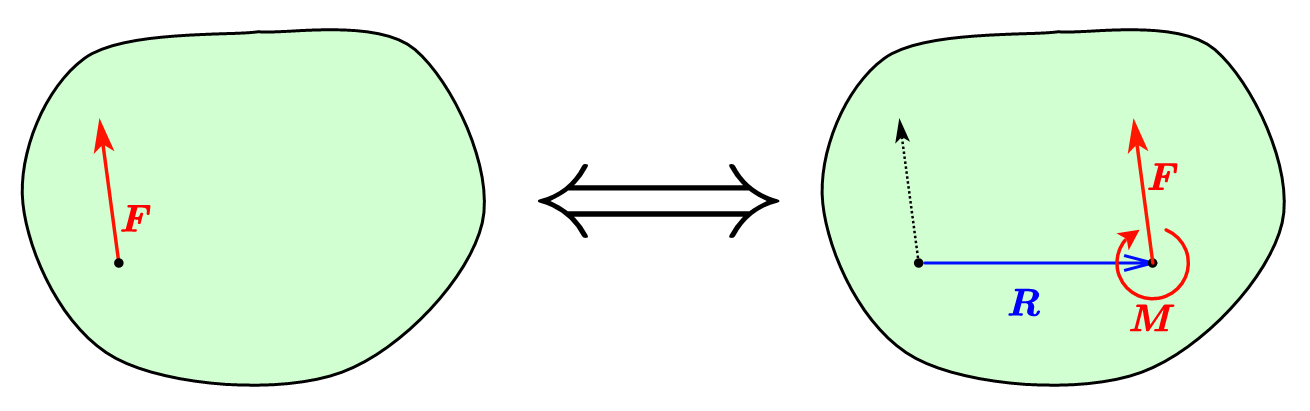
\includegraphics[width=10cm]{image/6-2-14.png}
\caption{力平移定理}
\end{figure}
即力平移以后的效果与原来的力的效果的区别可以被一个力偶等效.


如果力系简单,\,那么其平衡条件也是简单的.\,二力平衡条件就是等大,\,反向,\,共线.\,而三力平衡条件也相对简单实用,\,就是三力汇交,\,力三角两个条件.

\[\text{推论五}:\qquad \text{三力平衡条件}:\,\text{三力作用线三线共点,\,且三力首尾相连构成闭合三角形.}\]

\begin{wrapfigure}[5]{o}[-10pt]{6cm}
\vspace{-0.8cm}
\centering
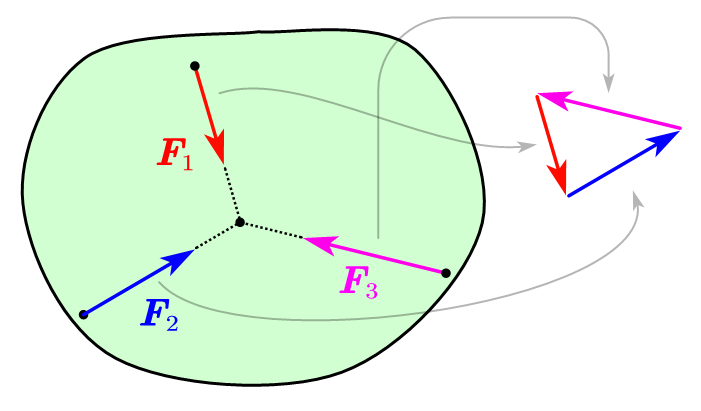
\includegraphics[width=6cm]{image/6-2-15.png}
\caption{三力汇交力三角}
\end{wrapfigure}
\vspace{1cm}
利用三力汇交可以把简单力系的平衡条件完全变成几何上的边角关系.\,而``力三角''的矢量三角形在很多具体的例子中也恰好与位形空间中的三角形相似,\,以提供一种完全几何化的解题思路.

\vspace{1.2cm}

\subsection{力系向一点简化}

利用强大的力平移定理,\,我们就可以实现力系向一点的简化.\,对于任意一个空间力系,\,在空间中取一点作为简化中心.\,那么就以这个点作为原点来写出每个力的作用点,\,力系被描述为:
\[\mathfrak{F}=\{\cdots(\bs{r}_i,\,\bs{F}_i)\cdots\}\]

但是又根据力平移定理:
\[(\bs{r}_i,\,\bs{F}_i)\equiv\{(\bs{0},\,\bs{F}_i),\,\bs{M}_i\}\quad,\quad \bs{M}_i=\bs{r}_i\times\bs{F}_i\]

故力系简化为:
\[\mathfrak{F}\equiv\{\cdots(\bs{0},\,\bs{F}_i)\cdots\bs{M}_i\cdots\}\]

再由共点力系求合力与力偶系求合力的方法:
\[\{\cdots(\bs{0},\,\bs{F}_i)\cdots\}\equiv(\bs{0},\,\bs{F})\]
\[\{\cdots\bs{M}_i\cdots\}\equiv\bs{M}\]

这个和称作力系对简化中心的\emph{主矢}(principal vector)与\emph{主矩}(principal moment):
\[\bs{F}=\sum_i\bs{F}_i\quad;\quad \bs{M}=\sum_i\bs{r}_i\times\bs{F}_i\]

其实,\,这样的结果可以推广到十分普遍的分布力系上来:
\[\bs{F}=\int\bs{f}\ud V\quad;\quad\bs{M}=\int\bs{r}\times\bs{f}\ud V\]

力系平衡的充要条件,\,是对任何一点主矢和主矩同时为零.\,也就是说有无数个彼此等价的条件.\,这些条件彼此之间有什么关系?\,这一点需要我们考察对不同点作简化的结果.\,事实上,\,如果力系对原点简化结果为:
\[\mathfrak{F}\equiv\{(\bs{0},\,\bs{F}),\,\bs{M}\}\]

那么换成位矢为$\bs{R}$的一点,\,简化结果一定为:
\[\mathfrak{F}\equiv\{(\bs{R},\,\bs{F}),\,\bs{M}-\bs{R}\times\bs{F}\}\]

也就是说,\,主矢是不会变的,\,只有主矩会变.\,从而主矢的不等于零是本质的,\,无法改变的.\,但是主矩的不等于零确是条件的.\,最后考虑若的确$\bs{F}\neq \bs{0}$,\,但当$\bs{R}$任取时,\,主矩上多出来的项$-\bs{R}\times\bs{F}$具有两个性质:\,一是必须与$\bs{F}$垂直,\,二是在与$\bs{F}$垂直的平面上可以取到任意值.\,我们还可以总结出平面力系与空间力系的最终简化结果:

\vspace{0.5cm}

\emph{平面力系的最终简化结果分类}:
\begin{itemize}
	\item 平衡力系:\,$\mathfrak{F}\equiv\mathfrak{0}$
	\item 单力:\,$\mathfrak{F}\equiv(\bs{r},\,\bs{F})$
	\item 单力偶:\,$\mathfrak{F}\equiv\bs{M}$
\end{itemize}

\vspace{0.5cm}

\emph{空间力系的最终简化结果分类}:
\begin{itemize}
	\item 平衡力系:\,$\mathfrak{F}\equiv\mathfrak{0}$
	\item 单力:\,$\mathfrak{F}\equiv(\bs{r},\,\bs{F})$
	\item 单力偶:\,$\mathfrak{F}\equiv\bs{M}$
	\item 力螺旋:\,$\mathfrak{F}\equiv\{(\bs{r},\,\bs{F}),\,\bs{M}\}$且$\bs{F}//\bs{M}$
\end{itemize}



\section{平衡问题:  矢量力学}

\subsection{平衡问题的要素}

在一个典型的平衡问题中,\,作为已知量未知量的可能要素如下所示.\,本节枚举中如果某要素只能为{\color{blue} 已知}则标{\color{blue} 蓝},\,如果只能为{\color{red} 未知}(即待求解的量)则标{\color{red} 红}.\,{\color{purple} 都可以}则标{\color{purple} 紫}.

\begin{itemize}
	\item {\color{blue} 体系的结构}:\,所有平衡问题中,\,体系的结构都是完全独立于其它量的已知未知提法的.\,它在确定其它量的已知未知前就已经被完全确定是已知的.\,它的内容包括:\,{\color{blue} 约束个数,\,约束方程形式,\,约束力个数与写法,\,自由度个数,\,平衡方程个数,\,平衡方程写法}.
	\item {\color{red} 约束力}:\,约束力从来不会在平衡问题中先行给出,\,它永远是待求解的,\,正因为如此我们称呼它们为被动力.\,其它所有力都与它们对立,\,称为主动力.
	\item {\color{purple} 主动力}:\,只要不是约束给出的力,\,原则上都视为主动力.\,但是不是所有主动力,\,在一个典型的平衡问题中都会事先给出.\,有些力,\,比如{\color{blue} 重力},\,总是已知.\,但是,\,比如一些问题问法就是求某外力等于多少时体系可以平衡;\,有些题目中出现弹簧的弹力,\,但是弹簧的伸长本身又是未知待求解的;\,动摩擦力,\,作为主动力,\,它依赖于未知的支持力;\,还有的题目干脆把约束解除,\,用未知的主动力代替原来也未知的约束力.\,这些情况下主动力也会变成未知力.
	\item {\color{purple} 位形变量}.\,很明确地,\,一个平衡问题分为两大类.\,一类问题(由于自由度为零或负)中每一个几何参量都在问题提出的事后都完全已知.\,但是另一类问题(自由度大于零)中,\,即使是平衡时的几何参量也是实现未知的,\,需要通过平衡条件加以求解.\,这里只指出这一种现象,\,如何分类见之后小节:\,负静定,\,静定与超静定.
\end{itemize}

\subsection{平衡条件与判据}

平衡方程,\,顾名思义,\,就是平衡时各个已知量,\,未知量之间要满足的具体数学方程.\,平衡方程可以分为三类:
\begin{enumerate}
	\item 平衡条件,\,具体列法见下.\,它可以同时包含位形变量,\,主动力和约束力三类已知未知量.
	\item 约束方程,\,即以前讨论过的几何上的约束关系.\,它只包含位形变量一类未知量.
	\item 主动力的结构性方程,\,有一些未知的主动力实际上是由一定的结构导致的,\,弹簧上的力和动摩擦力就是典型的例子,\,它们都有一些计算公式.\,这样的方程也可以同时包含位形变量,\,主动力和约束力三类已知未知量.
\end{enumerate}

第一类方程,\,也就是\emph{平衡条件}(condition of equilibrium)无疑是平衡问题中最丰富的一类方程.\,具体问题中它却往往有很多种列法,\,并造成或简单或复杂的求解过程.\,这些条件中最基础的一类就是单个质点和刚体的平衡条件.\,它们分别为:
\vspace{1cm}

A.\,质点沿$l$方向的力平衡条件:\,质点上的主动力与被动力构成共点力系$\{\cdots\bs{F}_i\cdots\}$,\,任意选取某方向$l$的单位矢量$\bs{e}_l$以后有:
\[\sum_i\bs{e}_l\cdot\bs{F}_i=0\]

B.\,刚体沿$l$方向的力平衡条件:\,刚体受到主动力和被动力构成空间力系$\{\cdots(\bs{r}_i,\,\bs{F}_i)\cdots\}$,\,任意选取某方向$l$的单位矢量$\bs{e}_l$作为投影方向,\,平衡条件为:
\[\sum_i\bs{e}_l\cdot\bs{F}_i=0\]

C.\,刚体绕$\bs{R}$点沿$l$方向的力矩平衡条件:\,刚体受到主动力和被动力构成空间力系$\{\cdots(\bs{r}_i,\,\bs{F}_i)\cdots\}$,\,任意选取位矢为$\bs{R}$的点作为矩心,\,任意选取某方向$l$的单位矢量$\bs{e}_l$作为投影方向,\,平衡条件为:
\[\sum_i\bs{e}_l\cdot[(\bs{r}_i-\bs{R})\times\bs{F}_i]=0\]

\vspace{1cm}
在三类平衡条件中,\,对一个具体的问题,\,由于$l$方向与$\bs{R}$点选取的任意性,\,平衡条件的列法都是无穷无尽的,\,但这不一定意味着这些所有方程都是\emph{独立}(independent)的,\,也就是说往往只列出少数几个就能充分地包含每一种列法的正确性.\,还有就是也不是所有列法在解决问题上都是同等简易的,\,比如为了使得某个未知力不出现在方程中以减少未知数和方程的个数,\,一方面利用\emph{整体法}(integral method)来消灭内力,\,一方面在列力平衡条件时选取垂直于力的方向作为投影方向,\,一方面列力矩平衡条件时选取力作用线上的点作为矩心.

以上三类方程还都属于\emph{隔离法}(isolation method)的平衡条件.\,事实上根据刚化原理,\,我们还可以把若干质点刚体看作整体,\,把作为内力的约束力忽略,\,列出整体法的平衡条件.\,容易理解这些平衡条件全都是隔离法平衡条件的组合,\,并不独立于隔离法的平衡条件.

于是一个重要的问题便浮现了出来,\,如何找到所有可能的平衡条件中,\,最少的,\,相互独立的,\,又能充分蕴含一切平衡条件的``核心平衡条件''?\,这些固定的平衡条件构成的组被称作\emph{平衡判据}(criterion of equilibrium).\,对这个问题的研究给出以下结果:

I.\,平面力系:

\quad A.\,质点的平衡判据
\[\left\{\begin{matrix}\displaystyle\sum_i\bs{e}_{l_1}\cdot\bs{F}_i=0 \\[1em] \displaystyle\sum_i\bs{e}_{l_2}\cdot\bs{F}_i=0\end{matrix}\right.\quad(\bs{e}_{l_1}\neq\pm\bs{e}_{l_2},\,\text{即两方向不平行})\]

\quad B.\,刚体的平衡判据
\[\left\{\begin{matrix}\displaystyle\sum_i\bs{e}_{l_1}\cdot\bs{F}_i=0 \\[1em] \displaystyle\sum_i\bs{e}_{l_2}\cdot\bs{F}_i=0\\[1em] \displaystyle\sum_i(\bs{r}_{i}-\bs{R})\times\bs{F}_i\footnote{力矩都在垂直平面方向.}=\bs{0}\end{matrix}\right.\quad(\bs{e}_{l_1}\neq\pm\bs{e}_{l_2},\,\text{即两方向不平行})\]
\[\left\{\begin{matrix}\displaystyle\sum_i\bs{e}_{l}\cdot\bs{F}_i=0 \\[1em] \displaystyle\sum_i(\bs{r}_{i}-\bs{R}_1)\times\bs{F}_i=\bs{0}\\[1em] \displaystyle\sum_i(\bs{r}_{i}-\bs{R}_2)\times\bs{F}_i=\bs{0}\end{matrix}\right.\quad(\bs{e}_{l}\cdot(\bs{R}_1-\bs{R}_2)\neq 0,\,\text{即矩心连线不能垂直于力投影方向})\]
\[\left\{\begin{matrix}\displaystyle\sum_i(\bs{r}_{i}-\bs{R}_1)\times\bs{F}_i=\bs{0} \\[1em] \displaystyle\sum_i(\bs{r}_{i}-\bs{R}_2)\times\bs{F}_i=\bs{0}\\[1em] \displaystyle\sum_i(\bs{r}_{i}-\bs{R}_3)\times\bs{F}_i=\bs{0}\end{matrix}\right.\quad(\text{三矩心不共线})\]

II.\,空间力系:
\quad A.\,质点的平衡判据
\[\left\{\begin{matrix}\displaystyle\sum_i\bs{e}_{l_1}\cdot\bs{F}_i=0 \\[1em] \displaystyle\sum_i\bs{e}_{l_2}\cdot\bs{F}_i=0 \\[1em] \displaystyle\sum_i\bs{e}_{l_3}\cdot\bs{F}_i=0\end{matrix}\right.\quad(\text{三投影方向不共面})\]

\quad B.\,刚体\footnote{本条均指非线状刚体.}的平衡判据
\[\left\{\begin{matrix}\displaystyle\sum_i\bs{e}_{l_1}\cdot\bs{F}_i=0 \\[1em] \displaystyle\sum_i\bs{e}_{l_2}\cdot\bs{F}_i=0\\[1em] \displaystyle\sum_i\bs{e}_{l_3}\cdot\bs{F}_i=0 \\[1em] \displaystyle\sum_i\bs{e}_{l_4}\cdot[(\bs{r}_{i}-\bs{R}_1)\times\bs{F}_i]=0 \\[1em] \displaystyle\sum_i\bs{e}_{l_5}\cdot[(\bs{r}_{i}-\bs{R}_2)\times\bs{F}_i]=0 \\[1em] \displaystyle\sum_i\bs{e}_{l_6}\cdot[(\bs{r}_{i}-\bs{R}_3)\times\bs{F}_i]=0\end{matrix}\right.\quad(\text{三力投影方向,\,三力矩投影方向都不共面})\]
\[\cdots\footnote{还有2力+4力矩,\,1力+5力矩,\,6力矩三类平衡判据,\,在此略去.}\]

我们发现,\,质点和刚体的平衡判据的方程个数都是严格等于无约束情况下各自的自由度数的:\,平面问题质点是2而刚体是3,\,空间问题质点是3而刚体是6.\,线状刚体,\,其力系也会具有共轴的特征,\,读者可以证明,\,此时空间问题中无论如何书写独立的方程数也将退化为5.

\vspace{1cm}
平衡问题复杂,\,多变.\,牛顿矢量力学情况下有没有万全的求解套路呢?\,对于一部分问题是有的,\,这给出了:

\subsection{亚静定,  静定与超静定}

单独考虑约束方程与位形变量之间的关系是任何平衡问题的分类过程中首当其冲的.\,参考之前对自由度与约束的讨论.\,一个体系若包含$a$个质点,\,$b$个线状刚体,\,$c$个非线状刚体,\,没有任何约束前自由度为$s=3a+5b+6c$.\,至此我们已经知道了一点,\,完全利用隔离法,\,可以列的平衡方程就是所有物体的平衡判据组合在一起,\,一共也是$s=3a+5b+6c$个方程.

这时候就开始分为三种典型的情形:

\begin{enumerate}
	\item 体系具有$r<s$个约束.\,首先,\,增添$r$个约束方程,\,那么体系剩余自由度为$f=s-r$,\,这就是说凭约束方程不足以解出平衡时的位形变量.\,称作\emph{亚静定问题}(hypo-statically-determinate problem).\,其次,\,此时待解未知数至少有$f$个剩余独立位形变量,\,和$r$个约束带来的约束力.\,但\emph{如果所有主动力已知},\,那么,\,刚刚好就能够用$s$个平衡方程求解出所有未知数来.\,如果$f$个独立的位形变量作为已知量由问题事先给定,\,那么方程多而未知数少,\,就有可能发生无解的情况,\,这实际上就代表着体系无法平衡,\,自由度开始演化,\,问题就从静力学问题转变为了动力学问题.\,也就是可能发生``不静''的情况.
	\item 体系恰好具有$r=s$个约束.\,那么,\,不同于上一种情况,\,平衡时的位形变量就可以被完全确定下来.\,就是说体系处于绝对的``静''的状态.\,称作\emph{静定问题}(statically-determinate problem).\,其次,\,$s$个约束带来的约束力,\,\emph{在已知所有主动力的前提下},\,恰好可以用$s$个平衡方程求解$s$个约束力.\,这就是``定''的来源.
	\item 体系具有$r>s$个约束.\,那么约束方程显然是随自洽但冗余(不独立)的.\,相同于上一种情况的是,\,体系没有自由度了,\,处于绝对的``静''的状态.\,称作\emph{超静定问题}(hyper-statically-determinate problem).\,这是因为,\,不同于上一种情况的是,\,体系将存在$r$个未知约束力,\,已经超过可列的所有平衡方程的个数$s$了.\,这会导致约束力不确定,\,存在多解的情况.\,此时体系平衡是一定可以实现的.\,毕竟体系平衡定义为任意一组解能导致各部分即可.\,但是由于多解性,\,它其实是``不定''.\,所以这一类问题又被称作\emph{静不定问题}(statically-indeterminate problem).
\end{enumerate}

静不定问题常见于带静摩擦的平衡问题中,\,此时支持力和静摩擦力都是约束力,\,带来的约束较多.\,摩擦力由于解不唯一往往有一个范围,\,那么范围中的最小静摩擦力小于接触点的临界静摩擦力就成为了必要的平衡条件.\,实际解题过程中往往还结合摩擦角,\,摩擦锥等几何化方法进行求解,\,在此不再赘述.


\section{平衡问题:  虚功原理}

在一个平衡问题中,\,如果想对它进行分析力学化,\,那么需要对体系进行较简单的抽象.

我们考虑一个包含$a$个质点,\,$b$个线状刚体,\,$c$个非线状刚体的体系,\,初始自由度为$s=3a+5b+6c$.\,加上$r$个约束.\,那么自由度和广义坐标的个数都是$f=s-r$,\,不妨设广义坐标为$q_1,\,q_2\cdots q_n$.\,再施加若干主动力.\,这些主动力要么作用于质点上,\,要么作用于刚体的某点上.\,而约束将能给出:\,任意一个点的坐标都可以用$f$个广义坐标来表述:
\[\bs{r}_k=\bs{r}_k(q_i,\,t)\quad i=1,\,2\cdots f\]

反过来理解,\,约束方程本身又是对那些点的坐标,\,进行限制,\,也就是说下面$r$个约束方程也能反映约束:
\[f_j(x_k,\,y_k,\,z_k,\,t)=0\quad j=1,\,2\cdots r\]

现在既然是静力学,\,我们就多提一点要求:\,以上两组方程都不能随时间变化:
\[\bs{r}_k=\bs{r}_k(q_i)\quad;\quad f_j(x_k,\,y_k,\,z_k)=0\]

这样我们就可以引入\emph{虚位移}(virtual displacement)这一概念的初等理解方式.\,它就是指在平衡位置附近假想的位移(坐标改变),\,发生位移了以后不一定还能平衡,\,这很显然.\,但是这个位移决不能破坏约束.\,即:
\[\delta \bs{r}_k=\sum_i \frac{\partial \bs{r}_k}{\partial q_i}\delta q_i \quad;\quad \sum_k\left(\frac{\partial f_j}{\partial x_k}\delta x_k+\frac{\partial f_j}{\partial y_k}\delta y_k+\frac{\partial f_j}{\partial z_k}\delta z_k\right)=0\]

另一个要求,\,彻底决定了约束力的性质,\,让平衡问题成为分析力学中非常简单的一类问题.\,就是关于约束必须是理想约束的要求:

\subsection{理想约束}

定义方法一:\,如果约束力总是可以通过约束方程来如此计算,\,那么约束就是理想约束:
\[R_{kx}=\lambda \frac{\partial f_j}{\partial x_k}\quad,\quad R_{ky}=\lambda \frac{\partial f_j}{\partial y_k}\quad,\quad R_{kz}=\lambda \frac{\partial f_j}{\partial z_k}\]

定义方法二:\,如果约束力永远不做虚功,\,那么约束就是理想约束:
\[\forall \delta \bs{r}_k,\,\sum_k \bs{R}_k\cdot \delta \bs{r}_k=0\]

结合对$\delta \bs{r}_k$需要满足的约束方程来看,\,以上两种定义方法的等价性是不言自明的.

值得注意的是,\,根据之前引入的广义力的说法,\,如果把作用在各个质点和刚体上的点上的约束力来求对各个广义坐标的广义力:
\[Q_{Ri}=\sum_k \bs{R}_k\cdot \frac{\partial \bs{r}_k}{\partial q_i}\]

又根据理想约束的定义,\,其虚功为零,\,但具有这样的算法:
\[\delta W_R=0=\sum_k \bs{R}_k\cdot \delta \bs{r}_k=\sum_k \bs{R}_k\cdot \sum_i \frac{\partial \bs{r}_k}{\partial q_i}\delta q_i=\sum_i\left(\sum_k \bs{R}_k\cdot \frac{\partial \bs{r}_k}{\partial q_i}\right)\delta q_i=\sum_i Q_{Ri}\delta q_i\]

由于对任意虚位移$\forall\delta q_i$上式都成立,\,这就得到了:
\[Q_{Ri}=0\]

所以理想约束的约束力只会作为内力而存在,\,其在每一个广义坐标上都没有任何广义力以影响这个自由度的运动.\,广义坐标的选取本身就是一个隐藏内部约束效果的结果.



\subsection{亚静定问题的虚功原理}

上述讨论的情形实际上就是亚静定问题.\,现在的平衡问题平衡条件就可以得到一个更简单的阐述.\,既然无论质点还是刚体上,\,考虑了主动力和约束力以后其合力都是零.\,那么在发生一个虚位移时,\,所有这些力做的总功都必然是零:
\[\delta W+\delta W_R=0 \]

既然现在是虚位移,\,约束力的虚功一定是零,\,那么主动力的虚功必然也有:
\[\delta W=0\]

这其实就已经构成平衡条件了.\,而它就是\emph{虚功原理}(principle of virtual work):\,一个理想约束系平衡时,\,主动力的虚功和必然是零.

而如果找到主动力在每一个自由度上的广义力,\,上式还可以被表述地更加具体:
\[Q_i=\sum_k \bs{F}_k\cdot \frac{\partial \bs{r}_k}{\partial q_i}=0\]

与矢量力学做比较,\,对于亚静定问题,\,矢量力学用$s$个平衡条件求解出$r$个约束你和$f$个位形变量.\,但是分析力学,\,直接用以上$f$个广义力为零的方程求解出$f$个位形变量,\,即广义坐标的平衡位置的值来.\,对问题的简化可见一斑.

\subsection{静定问题的求解}

对于静定问题以上方法也完全具有求解各个约束力的过程.\,如果要求解某一个约束上的约束力,\,那么就解除这一个约束,\,新的体系就成为一个亚静定的体系了.\,此时把原来根据约束方程确定的约束力(未知大小)换成主动力,\,如果一共解除了$f$个约束,\,就会出现$f$个未知的主动力,\,新的体系的广义坐标其实反倒是继承了原来静定问题的广义坐标值,\,是已知的,\,无需求解的.\,从而依然是未知的$f$个主动力在$f$个自由度上的广义力为零:
\[Q_i=0\]

就能够通过$f$个方程求解出原来的$f$个约束力来.

\section{分析力学初步*}

经过上一节对虚功原理的探讨,\,我们察觉到了分析力学理论建立的最基本条件:\,约束必须是理想的.\,但是与矢量力学方便处理的情况不同的是,\,理想的约束不一定是稳定的,\,此时分析力学照样也能够处理.

这就是说,\,与上一节相同,\,考虑一个包含$a$个质点,\,$b$个线状刚体,\,$c$个非线状刚体的体系,\,初始自由度为$s=3a+5b+6c$.\,加上$r$个约束.\,那么自由度和广义坐标的个数都是$f=s-r$,\,不妨设广义坐标为$q_1,\,q_2\cdots q_n$.\,再施加若干主动力.\,这些主动力要么作用于质点上,\,要么作用于刚体的某点上.\,而约束将能给出两组不同表述的方程:
\[\bs{r}_k=\bs{r}_k(q_i,\,t)\quad i=1,\,2\cdots f\]
\[f_j(x_k,\,y_k,\,z_k,\,t)=0\quad j=1,\,2\cdots r\]

\begin{wrapfigure}[13]{o}[-10pt]{5cm}
\vspace{-0.8cm}
\centering
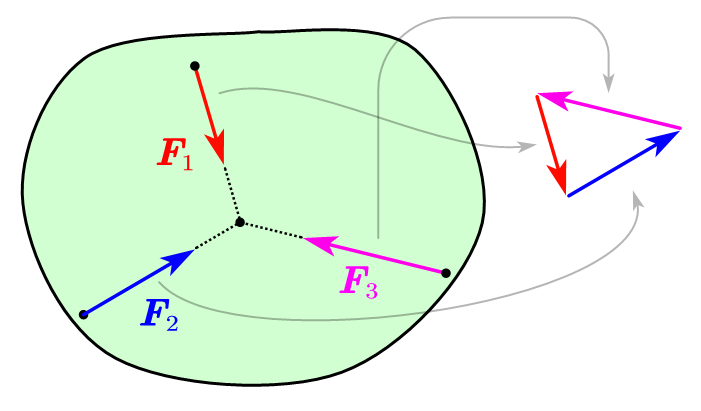
\includegraphics[width=5cm]{image/6-2-16.png}
\caption{实位移与虚位移}\label{fig:6-2-16}
\end{wrapfigure}
不同点在于,\,现在根本不需要以上方程不含$t$,\,下面的过程都是照推无误的.\,现在对于这样的非稳定约束,\,我们依然希望这样的约束不做虚功,\,不过此时的虚位移该如何表述?

在任何一个实际发生的动力学过程中,\,确定每个广义坐标的值就确定了在某一时刻的体系的位形,\,确定每个广义坐标随着时间的演化实际上就确定了一个具体的过程.\,而每一个质点在这样的具体的过程发生的实际位移就是\emph{实位移}(real displacement).\,它们应该满足:
\[\ud \bs{r}_k=\sum_i \frac{\partial \bs{r}_k}{\partial q_i}\ud q_i+\frac{\partial \bs{r}_k}{\partial t}\ud t\]
\[\sum_k\left(\frac{\partial f_j}{\partial x_k}\ud x_k+\frac{\partial f_j}{\partial y_k}\ud y_k+\frac{\partial f_j}{\partial z_k}\ud z_k\right)+\frac{\partial f_j}{\partial t}\ud t=0\]

那虚位移又以何种形式存在?\,回忆光学中的费马原理\footnote{它与分析力学的理论是同源的.}我们就可以找到答案:\,比如一个粒子做平抛运动\ref{fig:6-2-16}从$A$到达$B$.\,那么蓝色的轨迹就是粒子的实位移$\bs{r}(t)$,\,但是如果我们设想一条并不符合动力学规律,\,仅仅符合运动学约束的灰色轨迹,\,其运动方程为$\bs{r}'(t)=\bs{r}(t)+\bs{\delta}(t)$,\,那么这一条新的运动相对原来的运动的偏移就是虚位移$\bs{\delta}(t)$.\,对应到之前的情形,\,就是说在同一时间,\,约束的方程对原来正确的符合动力学规律的运动和虚位移以后的运动是同样成立的:
\[\bs{r}_k=\bs{r}_k(q_i,\,t)\quad,\quad f_j(x_k,\,y_k,\,z_k,\,t)=0\]
\[\bs{r}_k'=\bs{r}_k(q_i',\,t)\quad,\quad f_j(x_k',\,y_k',\,z_k',\,t)=0\]

用下式减上式,\,就得到了:
\[\delta \bs{r}_k=\sum_i \frac{\partial \bs{r}_k}{\partial q_i}\delta q_i\quad,\quad \sum_k\left(\frac{\partial f_j}{\partial x_k}\delta x_k+\frac{\partial f_j}{\partial y_k}\delta y_k+\frac{\partial f_j}{\partial z_k}\delta z_k\right)=0\]

这和$t$作为常数的稳定约束对运动的限制才是一致了.\,下一步,\,自然时要求约束力不能做虚功,\,注意,\,理想的却不稳定的约束情形中,\,约束力是可以做实功的,\,从而体系能量一般都不会守恒.\,总之,\,所谓理想约束,\,依然指的是:
\[R_{kx}=\lambda \frac{\partial f_j}{\partial x_k}\quad,\quad R_{ky}=\lambda \frac{\partial f_j}{\partial y_k}\quad,\quad R_{kz}=\lambda \frac{\partial f_j}{\partial z_k}\]
\[\forall\delta \bs{r}_k,\, \delta W_R=\sum_k \bs{R}_k\cdot \delta \bs{r}_k=0\]

最后只需解决主动力如何描述,\,最终重要的其实是主动力造成的广义力.\,也就是说我们计算以下量并以之描述所有主动力造成的``效果'':
\[Q_i=\sum_k \bs{F}_k\cdot \frac{\partial \bs{r}_k}{\partial q_i}\]


\subsection{用广义坐标表示能量}

一个体系最终会具有的能量,\,主要包括动能和势能.\,我们分别来研究两者:

\subsubsection{动能}
一个体系如果还包含刚体,\,那么其实总动能应当体现为:
\[T=\sum_k \frac{1}{2}m_k \bs{v}_k^2+\sum_l\frac{1}{2}\bs{\omega}_l\cdot \mathbb{I}_l\cdot \bs{\omega}_l\]

这里不可避免地需要使用到以后引入的刚体的惯量张量$\mathbb{I}_l$的概念.\,为了简化问题,\,我们可以考虑把刚体也抽象为带约束的质点系,\,那么只需要写出:
\[T=\sum_k \frac{1}{2}m_k \bs{v}_k^2\]

就注意表达任意复杂体系的动能函数.\,现在我们来进行广义坐标化.\,利用上一小节给出的:
\[\ud \bs{r}_k=\sum_i \frac{\partial \bs{r}_k}{\partial q_i}\ud q_i+\frac{\partial \bs{r}_k}{\partial t}\ud t\]

等号两侧同时除$\ud t$,\,得到质点速度的广义坐标表达法:
\[\bs{v}_k=\sum_i \frac{\partial \bs{r}_k}{\partial q_i}\dot{q_i} +\frac{\partial \bs{r}_k}{\partial t}\]

带回动能表达式,\,我们得到:
\[T=\sum_i\sum_j\sum_k\frac{1}{2}m_k\frac{\partial \bs{r}_k}{\partial q_i}\cdot\frac{\partial \bs{r}_k}{\partial q_j}\dot{q_i}\dot{q_j}+\sum_i\sum_k m_k\frac{\partial \bs{r}_k}{\partial q_i}\cdot\frac{\partial \bs{r}_k}{\partial t}\dot{q_i}+\sum_k \frac{1}{2}m_k\left(\frac{\partial \bs{r}_k}{\partial t}\right)^2\]

这就是说,\,动能可以分解广义速度$\dot{q_i}$的二次齐次项$T_2$,\,一次齐次项$T_1$,\,和随时间变的常数项$T_0$的和:
\[T=T_2+T_1+T_0\]
\[T_2=\sum_i\sum_j A_{ij}\dot{q_i}\dot{q_j}\quad,\quad A_{ij}=\frac{1}{2}\sum_k m_k\frac{\partial \bs{r}_k}{\partial q_i}\cdot\frac{\partial \bs{r}_k}{\partial q_j}\]
\[T_1=\sum_i B_i \dot{q_i}\quad,\quad B_i=\sum_k m_k\frac{\partial \bs{r}_k}{\partial q_i}\cdot\frac{\partial \bs{r}_k}{\partial t}\]
\[T_0=C\quad,\quad C=\frac{1}{2}\sum_k m_k\left(\frac{\partial \bs{r}_k}{\partial t}\right)^2\]

如果体系包含的约束全都是稳定约束,\,那么一切关于$t$的偏导数消失,\,动能就只剩下二次齐次项了,\,即$T=T_2$.

我们再定义两个量,\,一个是与广义坐标$q_i$相伴相生的那些广义速度,\,广义加速度,\,广义力同系列的最后一个量:\,\emph{广义动量}(general momentum).\,它的定义始终为:
\[p_i=\frac{\partial T}{\partial \dot{q_i}}\]

也就是把实际的动能看作$\dot{q_i}$的至多二次多项式,\,而把下面的偏导数定义为与第$i$广义坐标$q_i$共轭的广义动量:
\[p_i=\frac{\partial}{\partial \dot{q_i}}\left(\sum_i\sum_j A_{ij}\dot{q_i}\dot{q_j}+\sum_i B_i \dot{q_i}+C\right)=2\sum_j A_{ij}\dot{q_j}+B_i\]

第二个量,\,在数学上称作\emph{勒让德变换}(Legendre transform),\,我们定义一个动能的变式:
\[U=\sum_i p_i\dot{q_i}-T\]

很容易验证,\,在以上三项分解法下,\,这个变式的动能其实为:
\[U=T_2-T_0\]

广义动量和变式动能的意义何在?\,至少从定义上考虑,\,$p_i\ud \dot{q_i}$将会是动能的实际改变中的一项,\,完整的写法为:
\[\ud T=\sum_i \frac{\partial T}{\partial q_i}\ud q_i+\sum_i \frac{\partial T}{\partial \dot{q_i}}\ud \dot{q_i}+\frac{\partial T}{\partial t}\ud t\]

三项中第二项就是$p_i\ud \dot{q_i}$.\,而外力做功中的对应项为$Q_i\ud q_i$,\,虽然两者不存在直接的等量关系,\,但是它们至少是同量纲的.\,现在即使让两者相等也得不到任何有意思的结果.\,这是因为这个动能函数还需要修正.\,如果考虑变式动能$U$,\,根据定义,\,有:
\[\ud U=-\sum_i \frac{\partial T}{\partial q_i}\ud q_i+\sum_i \dot{q_i}\ud p_i-\frac{\partial T}{\partial t}\ud t\]

乍一看这样的做法找不到经典力学中的对应,\,其实不然:\,经典力学中根本就不会有非稳定约束,\,从而$T=U=T_2$.\,所以在更普遍的情况下,\,用$U$在某些场合代替原来的$T$也是可以理解的.\,最关键是,\,如果设想让外力在$q_i$上做功转化为上式第二个求和项中对应项(注意下式是错误的结论,\,仅仅是一种在特殊情况下成立的设想):
\[Q_i\ud q_i=\dot{q_i}\ud p_i=\frac{\ud q_i \ud p_i}{\ud t}=\dot{p_i}\ud q_i\quad\Rightarrow\quad Q_i=\dot{p_i}\]

这就是说,\,广义力的效果其实就是在改变对应自由度上的广义动量.\,这个说法后面却可以说明是对的,\,虽然上式不对,\,它漏项了.

\subsubsection{势能}

之前,\,我们简单地把体系中质点和刚体的受力二分为约束力(即被动力)和主动力.\,现在我们要重新观察众多种类的主动力中,\,保守力的可能性.\,有时候,\,体系内部的部分之间具有势能,\,带来非约束力的内力.\,有时候体系受到的外力也可以由势能来描述.\,多个势能函数直接求和,\,自然可以同时产生多个对应的保守力.\,从而我们定义,\,如果体系的所有主动力都有对应的势能,\,即都是保守力,\,那么体系称作\emph{保守}(conserved)的.\,也就是说,\,主动力全都由势能函数$V(\bs{r}_k)$描述:
\[\bs{F}_k=-\frac{\partial V}{\partial x_k}\bs{e}_x-\frac{\partial V}{\partial y_k}\bs{e}_y-\frac{\partial V}{\partial z_k}\bs{e}_z=-\nabla_k V\]

但是旋即便发现,\,如果用广义坐标表示$\bs{r}_k$并最终表示势能,\,在约束为非稳定约束情形下,\,势能将变成显含时间的形式$V(q_i,\,t)$.\,所以我们从一开时就默认最初势能也可以含有$t$,\,即$V(\bs{r}_k,\,t)$.\,对应的例子比如,\,在质量变化的太阳$M(t)$外距离为$r$的地球$m$的势能,\,就是:
\[V(\bs{r},\,t)=-\frac{GM(t)m}{r}\]

势能,\,以后都要理解为势能函数,\,作为一个数它不一定与动能的和守恒,\,但是上面这个势能至少可以告诉我们,\,地球的受力就是这个函数的负梯度:
\[\bs{F}(\bs{r},\,t)=-\nabla V=-\frac{GM(t)m}{r^2}\bs{e}_r\]

故现在,\,我们直接总结,\,保守体系的主动力部分,\,由势能函数$V(q_i,\,t)$来描述.\,十分容易验证的一点是,\,此时主动力在广义坐标上的广义力,\,也恰好可以通过负偏导数来计算:
\[Q_i=-\frac{\partial V}{\partial q_i}\]

但是一定要注意,\,由于势能本身就在随时间变化,\,故主动力做的实功并不会等于势能的降低,\,而是有:
\[-\ud V=\sum_i Q_i\ud q_i -\frac{\partial V}{\partial t}\ud t\]

反倒是在虚位移情形下,\,有
\[-\delta V=\sum_i Q_i\delta q_i\]


\subsection{拉格朗日方程}

至此,\,一个由广义坐标描述的,\,反映广义力是如何改变广义动量的严谨正确的最终方程就呼之欲出,\,只差临门一脚了.\,我们先不做任何体系上的主动力是否保守的假设,\,在一个十分普遍的问题中,\,每一个自由度$q_i$上的广义力为$Q_i$.\,最初我们只能知道每一个质点都符合牛顿定律:
\[\bs{R}_k+\bs{F}_k=m_k \ddot{\bs{r}}_k\]

如何从这个定律抽象到广义坐标呢?\,核心的问题是要解决$\ddot{\bs{r}}_k$的广义坐标化.\,为了将求导的阶数降低,\,我们构造真实路径$\bs{r}_k(t)$周围的虚位移以后的路径$\bs{r}_k(t)+\delta \bs{r}_k(t)$.\,一如既往地,\,虚位移要符合约束条件.\,而在牛顿定律两侧点乘虚位移,\,再来求和计算虚功和相伴产生的项:
\[\sum_k\bs{R}_k\cdot \delta \bs{r}_k+\sum_k\bs{F}_k\cdot \delta \bs{r}_k=\sum_k m_k \ddot{\bs{r}}_k\cdot \delta \bs{r}_k\]

第一项是约束力的虚功,\,由于是理想约束所以等于零.\,第二项才是真正的主动力虚功,\,用广义力和广义位移表示为$Q_i\delta q_i$的求和.\,第三项就是尚未算过的,\,这样处理也恰好提供了去除二阶导数的便利,\,从而方便广义坐标化:
\begin{align*}
\ddot{\bs{r}}_k\cdot \delta \bs{r}_k  	&=\sum_i\ddot{\bs{r}}_k\cdot \frac{\partial \bs{r}_k}{\partial q_i}\delta q_i\\
\ddot{\bs{r}}_k\cdot \frac{\partial \bs{r}_k}{\partial q_i}&=\frac{\ud }{\ud t}\left(\dot {\bs{r}}_k\cdot \frac{\partial \bs{r}_k}{\partial q_i}\right)- \dot {\bs{r}}_k\cdot \frac{\ud }{\ud t}\frac{\partial \bs{r}_k}{\partial q_i}\\
\sum_k m_k \ddot{\bs{r}}_k\cdot \delta \bs{r}_k&=\sum_i\left[\frac{\ud }{\ud t}\left(\sum_k m_k\dot {\bs{r}}_k\cdot \frac{\partial \bs{r}_k}{\partial q_i}\right)- \sum_k m_k\dot {\bs{r}}_k\cdot \frac{\ud }{\ud t}\frac{\partial \bs{r}_k}{\partial q_i}\right]\delta q_i
\end{align*}

现在我们暂时把动能写作:
\[T=\sum_k\frac{1}{2}m_k \dot {\bs{r}}_k^2\]

而其中$\dot {\bs{r}}_k$视作$q_i,\,\dot{q}_i$函数,\,有下列结论成立:
\[\frac{\partial T}{\partial q_i}=\sum_k m_k\dot {\bs{r}}_k\cdot \frac{\partial \dot {\bs{r}}_k}{\partial q_i}\]
\[\frac{\partial T}{\partial \dot{q}_i}=\sum_k m_k\dot {\bs{r}}_k\cdot \frac{\partial \dot {\bs{r}}_k}{\partial \dot{q}_i}\]
\[\dot {\bs{r}}_k=\sum_j\frac{\partial \bs{r}_k}{\partial q_j}\dot{q}_j+\frac{\partial \bs{r}_k}{\partial t}\quad\Rightarrow \quad \frac{\partial \dot {\bs{r}}_k}{\partial \dot{q}_i}=\frac{\partial \bs{r}_k}{\partial q_i}\]
\[\frac{\partial \dot {\bs{r}}_k}{\partial q_i}=\sum_j\frac{\partial^2 \bs{r}_k}{\partial q_i\partial q_j}\dot{q}_j+\frac{\partial^2 \bs{r}_k}{\partial q_i\partial t}\quad\Rightarrow \quad \frac{\ud }{\ud t}\frac{\partial \bs{r}_k}{\partial q_i}=\frac{\partial \dot {\bs{r}}_k}{\partial q_i}\]

后两式带入前两式并对比之前待化简的项,\,发现:
\[\sum_k m_k \ddot{\bs{r}}_k\cdot \delta \bs{r}_k=\sum_i\left[\frac{\ud }{\ud t}\left(\frac{\partial T}{\partial \dot{q}_i}\right)-\frac{\partial T}{\partial q_i}\right]\delta q_i\]

所以原来的牛顿定律,\,最后就变为:
\[Q_i=\frac{\ud }{\ud t}\left(\frac{\partial T}{\partial \dot{q}_i}\right)-\frac{\partial T}{\partial q_i}\]

这就是著名的\emph{拉格朗日方程}(Lagrange equation)的原型.\,也可以写成:
\[Q_i+\frac{\partial T}{\partial q_i}=\dot{p}_i\]

所以产生第$i$自由度上广义动量变化的原因除了广义力,\,还有一个动能本身对该自由度变化偏导数的因子.\,可以称做``几何力'',\,它的原因在于广义坐标与广义速度之间的耦合.

一个典型的例子比如在平面极坐标中研究粒子的运动,\,以矢径$r$和极角$\theta$为两自由度.\,矢量力学给出粒子受力$F_r,\,F_\theta$.\,但是粒子广义力为:
\[Q_r=F_r\quad,\quad Q_\theta=rF_\theta\]

写出动能:
\[T=\frac{1}{2}m(\dot{r}^2+r^2\dot{\theta}^2)\]

从而两个广义动量:
\[p_r=m\dot{r}\quad,\quad p_\theta=mr^2\dot{\theta}\]

后者即角动量.\,注意到在半径方向还有几何力:
\[\frac{\partial T}{\partial r}=m\dot{\theta}^2r\]

故拉格朗日方程,\,就变为:
\[F_r+m\dot{\theta}^2r=\frac{\ud}{\ud t}(m\dot{r})\quad ,\quad rF_\theta =\frac{\ud}{\ud t}(mr^2\dot{\theta})\]

这与矢量力学给出了一样的结果.

\vspace{1cm}
在体系为保守体系时,\,拉格朗日方程还可以获得一种更普遍的形式.\,只需要注意到势能函数,\,由于不能含有广义速度,\,与广义力之间符合以下关系:
\[Q_i=-\frac{\partial V}{\partial q_i}+\frac{\ud }{\ud t}\left(\frac{\partial V}{\partial \dot{q}_i}\right)\]

这样就得到了:
\[\frac{\ud }{\ud t}\frac{\partial (T-V)}{\partial \dot{q}_i}-\frac{\partial (T-V)}{\partial q_i}=0\]

一件令人震惊的事情就发生了:\,动能势能不是做和,\,而是做差,\,以函数的形式组合为了一个矢量力学中从未见过的新函数$L=T-V$.\,它就是著名的\emph{拉格朗日量}(Lagrangian).\,于是我们就遇到了标准的拉格朗日方程:
\[\frac{\ud }{\ud t}\frac{\partial L}{\partial \dot{q}_i}-\frac{\partial L}{\partial q_i}=0\]

对于$f$自由度系统拉格朗日方程也恰恰是$f$个,\,恰好能把问题解决.

在以上过程中,\,我们对势能的性质放松到了可以含有时间.\,这一步可以进一步放松.\,在有的场合下,\,拉格朗日量也是由两项构成,\,一项是常规意义下的动能,\,但是另一项势能也是含有速度的.\,这种势能函数叫做\emph{广义势能}(general potential energy).\,一种典型的情形是带点粒子在电磁场中运动的情形,\,此时动能势能为:
\[T=\frac{1}{2}m\dot{\bs{r}}^2\]
\[V=q(\varphi+\dot{\bs{r}}\cdot \bs{A})\]

其中$\varphi$是往往与电场对应的标势,\,$\bs{A}$则是往往与磁场对应的矢势.\,在这样的场合下,\,广义力的计算也要以下式为准:
\[Q_i=-\frac{\partial V}{\partial q_i}+\frac{\ud }{\ud t}\left(\frac{\partial V}{\partial \dot{q}_i}\right)\]

容易得到,\,最终粒子的拉格朗日方程,\,化简以后就是:
\[m\ddot{\bs{r}}=q\left[-\nabla\varphi+\frac{\partial \bs{A}}{\partial t}+\dot{\bs{r}}\times(\nabla\times\bs{A})\right]\]

故只要把电场,\,磁场视作:
\[\bs{E}=-\nabla\varphi+\frac{\partial \bs{A}}{\partial t}\quad,\quad \bs{B}=\nabla\times\bs{A}\]

就能给出正确的洛伦兹力公式和牛顿定律.\,以往在经典力学中与势能毫无关联的磁场力,\,分析力学下也是广义势能的结果.

\vspace{1cm}
最后我们来探讨守恒量的问题.\,用动能减势能这个操作固然不会得到什么守恒量,\,经典力学告诉我们保守系统守恒量应当是两者加起来,\,但是它导致了拉格朗日方程,\,以它为基础,\,我们能先后得到两个可能的守恒量.

一是在可能含有广义势的普遍情况下,\,广义动量被重新定义为:
\[p_i=\frac{\partial L}{\partial \dot{q}_i}\]

直接从拉格朗日方程可以看出,\,如果有
\[\frac{\partial L}{\partial {q}_i}=0\]

也就是拉格朗日量中不显含某个坐标$q_i$,\,这样的坐标称作\emph{循环坐标}(cyclic coordinate),\,那么这个自由度上的广义动量就不会随着时间改变.\,也就是``坐标平移不变导致动量守恒''.

二是,\,我们还记得之前引入过变式动能$U$,\,那么其实$U+V$才是对应经典力学中的总能量.\,或者,\,更普遍的,\,对任意拉格朗日量,\,定义\emph{哈密顿量}(Hamiltonian):
\[H=\sum_i p_i\dot{q}_i-L\]

那么直接计算其对时间导数就可以得到:
\[\frac{\ud H}{\ud t}=-\frac{\partial L}{\partial t}\]

从而如果拉格朗日量中不显含时间$t$\footnote{即使约束不稳定这也有可能发生.}.\,那么哈密顿量就会守恒.\,也就是``时间平移不变导致能量守恒''.


\subsection{再论冲击问题}

利用拉格朗日方程也可以求解碰撞问题.\,其实就是考虑拉格朗日方程的积分形式:
\[p_i'-p_i=\int \left(\frac{\partial T}{\partial q_i}+Q_i\right)\ud t\]

其中$p_i,\,p_i'$就是碰前碰后的广义动量,\,考虑到实际碰撞过程中几何力其实都是一些仅仅取决与广义坐标和广义速度的函数,\,过程中最多突变,\,但不会无限大,\,所以在极短时间内积分是趋于零的,\,而广义力积分给出了广义冲量$I_i$,\,它也正是各个主动力冲量(一般也就一个)$\bs{I}_k$计算的结果:
\[I_i=\sum_k \bs{I}_k\cdot \frac{\partial \bs{r}_k}{\partial q_i}\]


%\section{平衡态稳定性}

%\subsection{一自由度体系}



%\subsection{多自由度体系}


